\documentclass{article}
% Review version. Text: paper_review_text.md (author's text, used verbatim; only converted to LaTeX).
% NeurIPS 2025 style, preprint option; the style file is third-party and not in Git (run ../get_style.sh, then
% copy or link neurips_2025.sty here). Build: latexmk -pdf main_review.tex
\usepackage[preprint]{neurips_2025}

\usepackage[utf8]{inputenc}
\usepackage[T1]{fontenc}
\usepackage[hidelinks]{hyperref}
\usepackage{url}
\usepackage{booktabs}
\usepackage{amsfonts,amsmath,amssymb}
\usepackage{nicefrac}
\usepackage{microtype}
\usepackage{xcolor}
\usepackage{graphicx}
\usepackage{placeins}
\setcitestyle{authoryear,square,citesep={;},aysep={,}}

\title{Attention as Fast Weights: Reading, Diagnosing, and Correcting Attention Maps in Vision Transformers}

\author{Anonymous (course project, under review)}

\begin{document}
\maketitle

\begin{abstract}
Attention maps are the most common way to explain what a vision transformer (ViT) looks at, yet how to read them is rarely checked. We treat attention as a fast-weight network: for each image, fixed weights write a two-layer network whose hidden units are the tokens, so an attention map reads hidden activations. On DeiT-S, DeiT-B and DINO ViT-S, restricting every image region to the 16 units it reads keeps 72\%, 83\% and 61\% of top-1 predictions, against 9\%, 30\% and 4\% for random units. Of three premises behind the reading, two fail in deep layers: tokens lose their position in all models, and in supervised models a large activation is not a large contribution. Weighting each unit by its output contribution is the only correction that improves the map: in supervised ViTs it raises object focus and human alignment, beats removing high-norm tokens on object focus, and recovers 31--62\% of their last-layer drop. Relocating scores with position probes makes maps worse. Part of what makes deep attention maps look poor is how we read them.
\end{abstract}

\section{Introduction}

Attention maps are the most common window into what a vision transformer (ViT) \citep{dosovitskiy2021} attends to \citep{abnar2020,caron2021}. Two problems make them hard to trust. First, a map is a picture: it does not show that the model computes with the highlighted tokens \citep{jain2019,wiegreffe2019}. Second, agreement with human importance maps can be inflated by photographers' centre bias. In our setup, a fixed centred Gaussian that never looks at the image reaches a Spearman correlation of 0.41 with ClickMe human maps \citep{linsley2019}.

These problems matter most in deep layers. Attention maps of supervised ViTs become noisy and drift away from objects near the output \citep{darcet2024}, and the usual response is to change the model, for example by adding register tokens \citep{darcet2024,jiang2025}. We ask a different question: \textbf{how much of what makes an attention map look poor comes from how we read it, rather than from where the model looks?}

To make the reading itself testable, we revisit attention as a fast-weight network \citep{schmidhuber1992,schlag2021}. For each query, an attention head computes a two-layer network whose first-layer weights are the keys, whose activation is the softmax and whose second-layer weights are the values. The keys and values are written anew for each image by fixed (slow) projection weights. Each token is therefore a hidden unit, and an attention map is a reading of hidden activations drawn at the units' patch positions. This reading silently assumes three premises: the activations are specific to the image (M1), unit $j$ still stands for patch $j$ (M2), and a large activation means a large contribution (M3).

We use this lens to run one complete loop on three pretrained ViTs (DeiT-S, DeiT-B and DINO ViT-S), organised by three research questions. \textbf{RQ1 (read):} are the units read from attention used by the model? \textbf{RQ2 (diagnose):} where do the three premises fail? \textbf{RQ3 (correct):} can corrections derived from the lens improve the reading, and how do they compare with changing the model? Every correction is paired with a simpler stand-in that it must beat, all main metrics give zero credit to a centre prior, and all decision thresholds were fixed before the main runs.

Our contributions are:

\begin{enumerate}
\item \textbf{A lens whose reading is executable.} An execution test shows that the units read from attention are used: restricting each region to 16 of 197 units in all layers keeps most predictions, while random units do not.
\item \textbf{A diagnose--correct protocol with matched controls.} We measure each premise layer by layer and pair each lens-derived correction with a stand-in, under centre-controlled metrics.
\item \textbf{Findings on what can be fixed by reading.} Positional identity is lost in deep layers of all models, and activation differs from contribution in supervised models. Weighting attention by each unit's output contribution helps exactly where the second failure occurs, beats removing high-norm tokens on object enrichment, exceeds the gain from a test-time register (DeiT-S), and recovers 31--62\% of the last-layer degradation on these two metrics; relocating tokens with position probes makes maps worse, for reasons that four candidate explanations do not account for.
\end{enumerate}

Weighting attention by value-vector norms was proposed by \citet{kobayashi2020} for language models and used in ViT explanations by SNNA \citep{zhu2024}; we do not claim it as new. What is new is deriving it from the lens, testing it against a matched control and against model-side fixes, and predicting where it should not help.

\section{Related Work}

\textbf{Attention as explanation.} Whether attention explains predictions has long been debated \citep{jain2019,wiegreffe2019}. For transformers, attention rollout \citep{abnar2020} and gradient-weighted propagation (GAE) \citep{chefer2021} combine attention across layers, norm-based analyses weight attention by value-vector norms \citep{kobayashi2020,zhu2024}, and recent work filters ViT attention maps statistically \citep{ayyar2025}. Received attention also serves as a token-importance score in pruning \citep{goyal2020,kim2022}. Explanations are evaluated by deletion faithfulness \citep{bluecher2024} and by agreement with human maps \citep{fel2022}, and centre bias is known to confound saliency evaluation \citep{kuang2026}. \emph{Gap:} these works compare readings, but do not test the premises behind a reading, and human-alignment results for ViTs are rarely controlled for photographers' centre bias.

\textbf{Fast weights and attention as memory.} Linear attention is equivalent to fast-weight programming \citep{schmidhuber1992,schlag2021}, softmax attention is retrieval in a modern Hopfield network \citep{ramsauer2021}, and many sequence layers can be seen as test-time regressors \citep{wang2026}. Ramsauer et al.\ also measured how many tokens each BERT head averages over, and MiTA \citep{wen2026} trains models whose regions read only their top-$k$ keys. \emph{Gap:} the lens has been used to design or characterise models, not to audit how attention maps are read. We apply MiTA-style reading sets post hoc to standard ViTs as an execution test, and use the lens to derive the premises of a reading.

\textbf{Sinks, registers and token identity.} Supervised and large ViTs repurpose low-information patches as high-norm ``scratch'' tokens that attract attention \citep{darcet2024}; registers, trained or added at test time, take over this role \citep{darcet2024,jiang2025}, and attention sinks move rather than vanish \citep{fesser2026}. Deep tokens also lose their identity \citep{brunner2020}, become more similar to each other \citep{wang2022}, and absorb global semantics \citep{su2026}. \emph{Positioning:} we compare such model-side fixes with reading-side corrections on the same metrics, and test whether lost identity can be repaired by relocating scores.

\section{Methodology}

\begin{figure}[t]
\centering
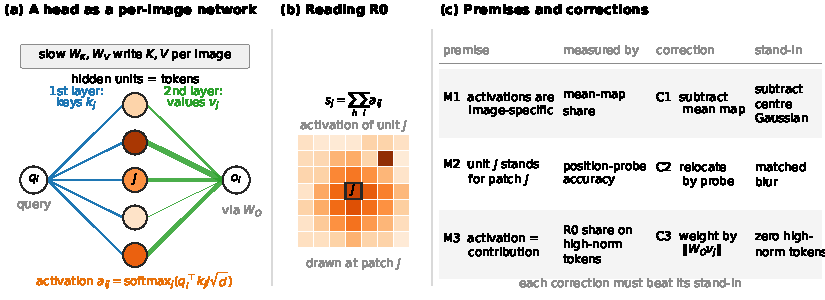
\includegraphics[width=\linewidth]{figure_1.pdf}
\caption{\emph{Attention as a fast-weight network.} (a) For each image, the slow weights write keys (first-layer weights) and values (second-layer weights); each token is a hidden unit. (b) An attention map reads the units' activations and draws unit $j$ at patch $j$. (c) The three premises of this reading (M1--M3), how each is measured, and the correction (C1--C3) and stand-in derived from it.}
\label{fig:lens}
\end{figure}

\subsection{Attention as a fast-weight network}

Let the 197 tokens entering block $\ell$ be the CLS token and 196 patch tokens. Head $h$ computes queries, keys and values by fixed projections, and for query $i$:
\begin{equation}
o_i = W_O^{h} \sum_{j} a_{ij} \, v_j, \qquad a_{ij} = \operatorname{softmax}_j\!\left(q_i^{\top} k_j / \sqrt{d_h}\right)
\end{equation}
Read as a function of the input $q_i$, this is a two-layer MLP: first-layer weights $\{k_j\}$, activation softmax, second-layer weights $\{v_j\}$, output projection $W_O^h$. The weights $K$ and $V$ are written anew for every image by the slow weights $W_Q$, $W_K$, $W_V$; they are fast weights, and token $j$ is hidden unit $j$. The standard ``attention received'' map reads the total activation of each unit and draws it at patch $j$:
\begin{equation}
s^{\ell}_j = \sum_{h} \sum_{i} a^{\ell h}_{ij}
\end{equation}
We call this reading \textbf{R0} and, unless stated otherwise, sum it over layers 9--12. Unlike in an MLP, softmax makes the units compete, so the analogy is approximate (Section 5).

\subsection{Read: reading sets and the execution test}

We split the $14\times14$ patch grid into 16 regions. Each region averages its queries, scores all keys, and keeps the top-$k$ as its reading set; CLS keeps its own top-$k$. We then rerun the model with every query allowed to attend only to its region's set, in all 12 layers at once, and record whether the top-1 prediction matches that of the unmodified model. Baselines are random sets of the same size (five seeds) and removing attention altogether; $k$ ranges from 4 to 128.

\subsection{Diagnose: three premises}

\begin{itemize}
\item \textbf{M1, the reading is image-specific.} We estimate the model's mean map $\bar s$ per layer on held-out images and report the share of within-image spatial variance it explains: one minus the variance of $s - \bar s$ over the variance of $s$, pooled over images.
\item \textbf{M2, unit $j$ stands for patch $j$.} A linear probe per layer predicts each token's original patch index (196 classes) from its representation after the block's first layer norm, which is the input to attention; we report top-1 accuracy on held-out images.
\item \textbf{M3, a large activation means a large contribution.} We report the share of R0 that falls on high-norm tokens: patches whose block-input norm exceeds three times the image's median at that layer.
\end{itemize}

\subsection{Correct: three corrections and their stand-ins}

Each premise gives one correction:
\begin{equation}
\text{C3: } c^{\ell}_j = \sum_{h}\sum_{i} a^{\ell h}_{ij}\,\lVert W_O^{h} v^{\ell h}_j \rVert_2 \qquad \text{C2: } r^{\ell}_p = \sum_j s^{\ell}_j \, P_\ell(p \mid x^{\ell}_j) \qquad \text{C1: } s^{\ell} - \bar{s}^{\ell}
\end{equation}
C3 (for M3) follows directly from the network view: a hidden unit's contribution is its activation times the size of its outgoing weight. C2 (for M2) moves each unit's score to where the probe says the unit now stands. C1 (for M1) removes the image-independent part. A correction could help for a simpler reason, so each has a \textbf{stand-in} it must beat: for C3, setting high-norm tokens to zero; for C2, a Gaussian blur whose mean squared displacement matches that of C2 in each layer; for C1, subtracting a centred Gaussian scaled to the mean map's spatial spread. The pre-registered combination of all three corrections is reported in Appendix D.

\subsection{Models, data and training}

We study frozen DeiT-S and DeiT-B \citep{touvron2021} and DINO ViT-S with its official linear head \citep{caron2021}, each with its own preprocessing. Two model-side variants are evaluated with the same protocol: DeiT-S with a test-time register that takes over the 8 FFN units producing high-norm tokens \citep{jiang2025}, and MiTA-DeiT-S trained with top-$k$ attention \citep{wen2026}. The only trained components are the 36 linear probes (12 layers $\times$ 3 models; Adam, learning rate 0.01, batch 4,096, 30 epochs, seed 0), trained on 2,000 held-out ImageNet validation images; another 2,000 held-out images give the mean maps and the probes' test accuracy. No held-out image is used for evaluation.

\section{Empirical Analysis}

\subsection{Experimental setting}

\textbf{Data.} The execution test uses a fixed set of 5,000 ImageNet validation images. Object alignment uses ImageNet-S \citep{gao2022}: all 12,419 images for enrichment (the metric is defined for 12,150 of them for DeiT-S and DeiT-B and 12,144 for DINO; the others have no valid object patch) and a fixed 2,000 for deletion. Human alignment uses the 17,408 released ClickMe maps \citep{linsley2019,fel2022}. We found that these images are very likely from the ImageNet \emph{training} set (only 2 of 4,002 held-out validation images reappear in them), so the models have seen them; we report ClickMe numbers with this caveat.

\textbf{Metrics.} \emph{Deletion faithfulness} is the SRG score of \citet{bluecher2024}: the area between the least- and most-important-first deletion curves. \emph{Same-ring object enrichment} compares the score on object and background patches at the same distance from the image centre. \emph{Image-specific human alignment} is the Spearman correlation with the image's own ClickMe map minus its correlation with the ClickMe map of the previous image in the same batch. Both alignment metrics give 0 to any map that does not depend on the image, such as a centred Gaussian, so a high score cannot come from centre bias alone. GAE \citep{chefer2021} is reported as a reference, not as a competitor: it uses gradients and class information that our readings do not.

\textbf{Statistics.} All differences are paired over images, with 1,000 bootstrap resamples (seed 0) and 95\% intervals. A difference counts as \emph{higher} or \emph{lower} only if its interval excludes 0 and it exceeds a margin fixed in advance (0.02; 0.05 for deletion); otherwise it counts as \emph{comparable}. Predictions, margins and the main comparisons were fixed before the runs (Appendix C); analyses added after seeing the main results are marked as exploratory. Two negative controls behave as predicted: C3 leaves DINO unchanged, and C2 leaves layers 1--4 unchanged (all absolute differences $\le$ 0.004). All readings pass the model-randomisation sanity check \citep{adebayo2018} (median Spearman to the original $\le$ 0.37 after full randomisation).

\subsection{RQ1: the units an attention map reads are the ones the model executes}

\textbf{Each region needs to read very few units, and the units the attention map picks are the right ones.} With $k = 16$ units per region (about 8\% of 196) in all 12 layers, the model keeps 72\% / 83\% / 61\% of its top-1 predictions (DeiT-S / DeiT-B / DINO). Random sets of the same size keep 9\% / 30\% / 4\%, and removing attention leaves 0.1\%--0.2\%. Reading sets beat random sets at every $k$ from 4 to 128 in every model (Figure~\ref{fig:read}a). Restricting one layer at a time costs much less (Appendix B): the test is strict because it changes all layers at once.

\textbf{The map is meaningful, but it is a weak heat map.} After centre bias is removed, R0 still prefers object patches (enrichment 0.140 / 0.080 / 0.199) and agrees with humans (0.157 / 0.107 / 0.208), while every image-independent reference scores about 0. GAE's mean is higher in all nine cells, by 0.022 to 0.138 (for example, deletion 0.345 vs 0.236 on DeiT-S). The next two sections ask why the gap exists.

\begin{figure}[t]
\centering
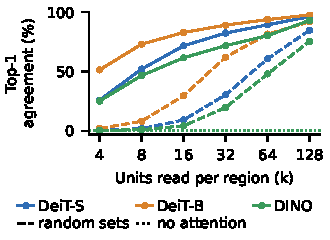
\includegraphics[height=3.9cm]{../../figures/figure_2a.pdf}\hfill
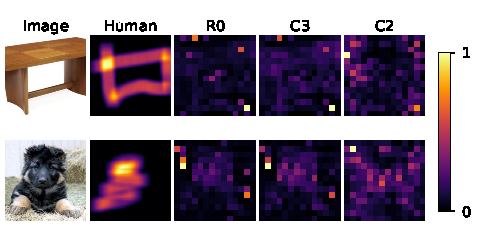
\includegraphics[height=3.9cm]{../../figures/figure_2b.pdf}
\caption{\emph{Read.} (a) Top-1 agreement with the unmodified model as the number of units read per region grows, for reading sets, random sets and no attention; three models. (b) Two ClickMe images drawn with a fixed seed, not selected: image, human map, R0, C3 and C2 (DeiT-S, layers 9--12, each map scaled to [0, 1]). Differences on single images are subtle; Table~\ref{tab:main} gives the aggregate. Layer 12 alone is in Appendix B.}
\label{fig:read}
\end{figure}

\subsection{RQ2: two of the three premises fail, in different places}

\textbf{Unit $j$ stops standing for patch $j$ in every model.} The linear probe recovers the patch index for almost every token in layers 1--5, then accuracy falls: 18\% / 32\% / 36\% at layer 12 (DeiT-S / DeiT-B / DINO).

\textbf{Large activation stops meaning large contribution, but only in supervised models.} In DeiT-B, 44\% of R0 at layer 11 falls on high-norm tokens; in DeiT-S, about 9\% at layers 8--10; in DINO, 0\% at every layer. These tokens have values on average only 0.23--0.29 times as long as ordinary patches (layers 9--12), so they receive attention but write little.

\textbf{The image-independent part is small.} The model's mean map explains only 3\%--6\% of the spatial variation in supervised layers 6--12, and up to 17\% in DINO layers 6--12. It is almost a set of concentric rings around the centre (in layers 9--12, 82\%--98\% of its variance is explained by distance from the centre).

No single premise lines up with the drop in R0's quality at the last layer (Figure~\ref{fig:diagnose}d): M2 declines smoothly, M3 peaks at layer 11 in DeiT-B, and in the supervised models M1 is smallest at layer 12. The premises describe \emph{where} the reading can mislead; whether fixing them helps is a separate, testable question.

\begin{figure}[t]
\centering
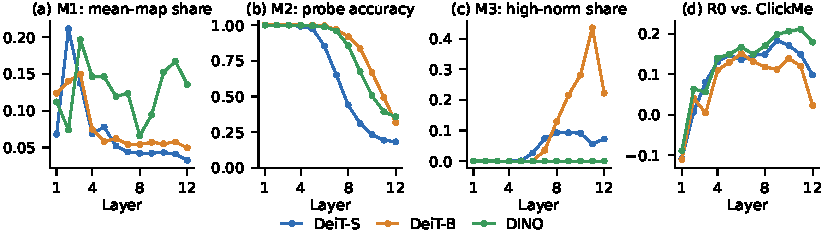
\includegraphics[width=\linewidth]{../../figures/figure_3.pdf}
\caption{\emph{Diagnose,} per layer for three models. (a) M1: share of spatial variance explained by the mean map. (b) M2: position-probe accuracy. (c) M3: share of R0 on high-norm tokens. (d) R0's image-specific ClickMe alignment.}
\label{fig:diagnose}
\end{figure}

\subsection{RQ3: only contribution weighting improves the reading}

\begin{table}[t]
\caption{Object enrichment / image-specific ClickMe alignment (layers 9--12; higher is better). Each correction is followed by its stand-in ($\llcorner$). 95\% intervals are at most $\pm$0.004 (enrichment) and $\pm$0.005 (ClickMe). Deletion scores, intervals and the combined readings are in Appendix D.}
\label{tab:main}
\centering
\small
\begin{tabular}{lccc}
\toprule
Reading & DeiT-S & DeiT-B & DINO \\
\midrule
Centre Gaussian & 0.000 / 0.000 & 0.000 / 0.000 & 0.000 / 0.000 \\
\textbf{R0} (attention received) & 0.140 / 0.157 & 0.080 / 0.107 & 0.199 / 0.208 \\
\textbf{C3} contribution weighting & \textbf{0.178 / 0.190} & \textbf{0.146 / 0.165} & 0.196 / 0.207 \\
\quad$\llcorner$ zero high-norm tokens & 0.152 / 0.168 & 0.121 / 0.148 & 0.199 / 0.208 \\
\textbf{C2} relocation by probe & 0.041 / 0.084 & 0.027 / 0.050 & 0.084 / 0.143 \\
\quad$\llcorner$ matched blur & 0.095 / 0.152 & $-$0.008 / 0.068 & 0.189 / 0.226 \\
\textbf{C1} subtract mean map & 0.138 / 0.165 & 0.077 / 0.087 & 0.201 / 0.252 \\
\quad$\llcorner$ subtract centre Gaussian & 0.133 / 0.168 & 0.056 / 0.062 & 0.200 / 0.253 \\
+ test-time register & 0.152 / 0.169 & --- & --- \\
top-$k$ training (MiTA) & 0.100 / 0.115 & --- & --- \\
GAE (reference) & 0.204 / 0.234 & 0.196 / 0.213 & 0.221 / 0.234 \\
\bottomrule
\end{tabular}
\end{table}

\textbf{C3 is the only correction that helps, and it helps where the lens says it should.} On both supervised models, C3 raises enrichment by +0.038 / +0.065 and ClickMe alignment by +0.033 / +0.058 (DeiT-S / DeiT-B), all \emph{higher}. It is more than removing the high-norm tokens: C3 beats that stand-in on enrichment in both models (+0.026 / +0.025) and on ClickMe in DeiT-S (+0.022). On DINO, which has no high-norm tokens, C3 changes nothing (all differences $\le$ 0.004), as predicted. On deletion, C3 is \emph{comparable} everywhere (+0.017 / +0.029 / 0.000). C3 also recovers 31\%--62\% of the last-layer drop in enrichment and ClickMe in the supervised models (8\%--29\% in deletion); no other correction recovers any (Appendix D). Three exploratory checks support this account (Appendix D). First, the gain comes from matching each unit with its own weight: shuffling the weights among tokens within a head, or replacing them by the head's mean, removes it entirely (C3 minus shuffled: +0.038 / +0.073 enrichment, +0.035 / +0.067 ClickMe). Second, the gain scales with the problem: images with more R0 mass on high-norm tokens gain more (Spearman with the ClickMe gain +0.045 / +0.158). Third, weighting by $\lVert v_j\rVert$ instead of $\lVert W_O v_j\rVert$ gives the same result, so in practice C3 reduces to value-norm weighting \citep{kobayashi2020}. C3 closes 57--59\% of the gap between R0 and GAE on enrichment and 43--54\% on ClickMe, but only 16--21\% on deletion. At single layers 8--11 of DeiT-B, zeroing high-norm tokens gains more than C3, and C3 gains more only at layer 12; C3's advantage appears when layers 9--12 are combined (Appendix D).

\textbf{C1 does nothing beyond removing centre bias.} It is \emph{comparable} to R0 on enrichment in all models. Its one gain, on DINO ClickMe (+0.044), is matched by subtracting a plain centred Gaussian (0.252 vs 0.253): because the mean map is almost radial, ``remove the image-independent part'' here means ``remove centre bias''. On DeiT-B, C1 is \emph{higher} than its stand-in on all three metrics, but only because subtracting a centred Gaussian falls below R0 there; C1 itself is not higher than R0 on any metric. This agrees with the small M1 share in Section 4.3.

\textbf{C2 makes every reading worse, usually worse than a blur of the same size.} C2 is \emph{lower} than R0 in all nine cells; for example, DINO enrichment falls from 0.199 to 0.084, while a blur that moves mass the same distance only lowers it to 0.189. So the probe does not just spread the score out; it sends the score to wrong places. The one exception is DeiT-B enrichment, where the blur itself falls below zero ($-$0.008) and C2 is higher than the blur, though still lower than R0. Section 4.5 asks why.

\textbf{Changing the model does not beat changing the reading.} A test-time register on DeiT-S is only \emph{comparable} to R0 (+0.012 / +0.013), against +0.038 / +0.033 for C3 on the same model. Training with top-$k$ attention (MiTA) is \emph{lower} ($-$0.040 / $-$0.042).

\textbf{Combining corrections is not robust.} The pre-registered order C3 $\to$ C2 $\to$ C1 is \emph{higher} than R0 in only one of four supervised cells (DeiT-B ClickMe, +0.030). The order C3 $\to$ C1 $\to$ C2 beats the pre-registered order in all nine cells, but we did not fix it in advance and base no claim on it. Adding C1 to C3 does not improve on C3 beyond our margins (enrichment $-$0.003 / 0.000, ClickMe +0.019 / +0.017), and adding C2 to C3 makes every cell worse. We therefore recommend C3 alone.

\subsection{Why does relocation fail?}

C2 fails although its premise fails, so we tested four simple explanations. All analyses in this section were added after the main results and are exploratory (Appendix E). None of the four meets its rule. \textbf{(i) Far errors.} Probe errors are mostly local: at layer 12, 45\% / 66\% / 81\% of the probe's probability lies within the $3\times3$ neighbourhood of the true patch (DeiT-S / DeiT-B / DINO), and only 4\%--29\% of its error mass lies more than three patches away. \textbf{(ii) A fixed positional prior.} The probe's average prediction is close to uniform (at layers 9--12 its peak is 1.1--1.3 times the uniform value) and is at most weakly related to the model's mean map. \textbf{(iii) A weak probe.} A two-layer MLP probe raises layer-12 accuracy by only 2--7 points, and C2 with this probe is still \emph{lower} than R0 in all six cells. \textbf{(iv) Global tokens.} Within a layer, the probe is not less certain about tokens that are more similar to the image's mean token; in all three models it is, if anything, more certain about them. Only in DeiT-B (layers 10--12) are these tokens placed less accurately, so the rule, which requires both lower accuracy and higher uncertainty, holds in no model.

What remains is a description, not a cause. On DeiT-S, C2 moves about as much score off the object as the matched blur (0.041 vs 0.039), yet lowers enrichment twice as much ($-$0.099 vs $-$0.045): it scatters each token's score irregularly over nearby patches and so scrambles their ranking, while a blur moves scores smoothly. Relocating only the tokens the probe is confident about (top probability $\ge$ 0.5) removes 37\%--94\% of the damage, but not all of it. Keeping each score in place but discounting it by the probe's probability that the unit is still at its patch does not help either: it is \emph{lower} than R0 in four of six cells and \emph{comparable} on DeiT-B, and in DeiT-S and DINO it is also lower than discounting by the same probabilities shuffled among tokens, on both metrics. This suggests that, in these models, the probe is less sure about the positions of object patches than of background patches. We conclude that relocation by position probes is not a safe correction, and we leave the mechanism behind M2's failure open.

\section{Discussion}

\textbf{Diagnosis predicts correction, in two of three cases.} The loop gives a simple check: a correction should help only where its premise fails, and only by more than its stand-in. This holds for two premises. M1 holds (the image-independent part is small), and C1 never improves on R0 except where subtracting a centred Gaussian gives the same gain. M3 fails only in supervised models, and C3 helps only there, on object enrichment by more than zeroing the high-norm tokens. M2 is the exception: it fails in every model, yet its correction hurts everywhere. A failed premise is therefore not enough; the correction must also match \emph{how} it fails. The probe's errors are mostly local, yet moving scores by its predictions still scrambles their ranking (Section 4.5).

\textbf{What this means in practice.} (i) When reading attention from a supervised ViT, weight each unit by its contribution, $\lVert W_O v_j\rVert$; it costs one norm per token and needs no gradients. (ii) Check a new correction against a stand-in of the same strength, not only against the uncorrected map: in our data, in every model a matched blur costs 0.029--0.049 less on ClickMe than on object enrichment, so a metric can reward smoothing. (iii) Do not read deep attention maps as ``patch $j$ is important''; in late layers (from layer 8 in DeiT-S, layer 11 in DeiT-B and DINO), the probe says unit $j$ often no longer stands for patch $j$.

\textbf{Limitations.} First, softmax makes the units compete, so attention is not exactly a two-layer MLP; our tests check what the analogy predicts, not that it is exact. Second, we study three ImageNet classifiers at sizes S and B, each from a single trained run. High-norm artefacts in DINOv2 appear only at ViT-L and above \citep{darcet2024}, so we could not test trained registers at our scale. Third, our position probes are linear or two-layer; other kinds of probe may find position information that ours miss. Fourth, the ClickMe images were very likely seen during training. Finally, our readings are class-independent and remain well below GAE; we aim to explain attention maps, not to replace gradient methods.

\textbf{Ethical considerations.} Better-looking explanations can raise trust in a model more than they should. We therefore report where every correction fails, compare each with a simple stand-in, and fix our tests in advance. We use only public models and datasets; the human maps were collected by \citet{linsley2019} under their own consent procedures.

\section{Conclusion}

Viewing an attention head as a per-image two-layer network turns attention maps into a reading of hidden units, with three premises that can be measured. The units this reading picks are the ones the model executes, but two premises fail in deep layers: tokens lose their patch identity in every model, and high-norm tokens absorb attention without contributing in supervised models. Only the correction for the second failure, weighting each unit by its contribution, improves the map; it beats its matched stand-in on object enrichment, and it helps only where that failure occurs.

\textbf{Future work.} Test the lens on larger models with trained registers (DINOv2 at ViT-L), replace the position probe with a reading that does not assume one place per token, and apply the same read--diagnose--correct loop to the FFN, which is also a two-layer network.

\textbf{Broader impact.} The fast/slow-weight view gives a common language for explaining what attention computes. Its main use is to warn when an attention map should not be trusted, and to give a cheap fix when it can be.

\bibliographystyle{plainnat}
\bibliography{references}

\FloatBarrier
\clearpage
% Appendices A-E of the paper. Tables are generated from the result files by make_appendix_tables.py.
\appendix
\setcounter{topnumber}{4}\setcounter{totalnumber}{6}
\renewcommand{\topfraction}{0.95}\renewcommand{\textfraction}{0.05}\renewcommand{\floatpagefraction}{0.75}

\FloatBarrier
\section{Implementation and reproducibility}
\label{app:impl}

\textbf{Code and reproduction.} Code, configurations, the fixed image lists and all result tables are in the accompanying repository (link withheld for anonymous review). Every table and figure is rebuilt from the saved run outputs by one command. A full rerun from a fresh copy of the repository in a fresh environment, on one NVIDIA L4 GPU (11.5 GPU hours), reproduced all 31 result tables: every verdict was identical, and the largest difference of a mean was $2.5\times10^{-5}$ (tolerance $10^{-4}$; $2\times10^{-3}$ for readings that use a retrained probe).

\textbf{Hardware and numerics.} PyTorch 2.7.0, timm 1.0.30, float32 without autocast, deterministic algorithms. All runs of the main protocol and all exploratory runs used NVIDIA L4 GPUs. Three groups of earlier runs that we reuse ran in part on an NVIDIA A100: the single-layer restriction (DeiT-B), head versus body patches, and the centre-Gaussian ClickMe number of Section~1. All runs together took about 19 GPU hours.

\textbf{Models and preprocessing.}
DeiT-S and DeiT-B are the supervised timm checkpoints \nolinkurl{deit_small_patch16_224.fb_in1k} and \nolinkurl{deit_base_patch16_224.fb_in1k} (pinned revisions), resize to 248 and centre crop 224 (crop ratio 0.9).
DINO ViT-S/16: timm \nolinkurl{vit_small_patch16_224.dino} with the official linear head (the CLS tokens of the last four blocks, concatenated), resize 256 and centre crop 224 (0.875).
MiTA-DeiT-S: the checkpoint released by the MiTA authors \citep{wen2026}, with its own evaluation transform (resize 256, crop 0.875); its row in Table~\ref{tab:main} is paired with DeiT-S by image, so the two models see slightly different crops of the same image.
The test-time register \citep{jiang2025} moves the activations of 8 FFN units of DeiT-S (layers 4 and 5) to one added token; the units were selected on 500 ImageNet-S pilot images that are not used for evaluation.
The no-attention baseline of Figure~\ref{fig:read}(a) and the single-layer removal column of Table~\ref{tab:single_layer} used a uniform transform for all models (resize 256, crop 0.875), so for DeiT-S and DeiT-B they used a 0.875 centre crop instead of their own 0.9 crop; the image indices are the same.

\textbf{Reading sets.} The $14\times14$ grid is pooled into 16 regions by $4\times4$ adaptive average pooling (windows $[0,4), [3,7), [7,11), [10,14)$ per axis). In every head, the mean query of each region is scored against all 197 keys and the top-$k$ keys form its reading set; each patch query is routed to its region by position, and CLS keeps its own top-$k$ set. The sets are computed in a forward pass of the unmodified model, then the model is rerun with a boolean attention mask. Random sets have the same size and routing (seeds 0--4, averaged per image). Before each run, an explicit-softmax implementation is checked against the model (same top-1 classes, largest logit difference $<5\times10^{-4}$).

\textbf{Diagnostics and corrections.} High-norm tokens are patches whose block-input norm exceeds three times the image's median at that layer. The position probes are linear (196 classes) on the output of the block's first layer norm, trained on all patch tokens of 2,000 held-out images (Adam, learning rate 0.01, batch 4,096, 30 epochs, seed 0); the two-layer MLP probe of Appendix~\ref{app:c2} is trained on 1,800 of these images with the other 200 for early stopping. The mean map $\bar s^\ell$ and the probe accuracy use another 2,000 held-out images; the held-out set excludes ImageNet-S images and ClickMe near-duplicates (2 of 4,002 candidates matched). The matched blur is an isotropic Gaussian whose mean squared displacement equals that of C2 at the same layer on held-out images. The centred-Gaussian stand-in of C1 is scaled to the mean map's spatial spread.

\textbf{Statistics.} Every difference is paired over images; intervals are 2.5th and 97.5th percentiles of 1,000 bootstrap resamples of the images (seed 0). The verdict rule and its margins are given in Section~4.1.

\textbf{AI assistance.} Code and experiments were run with an AI coding assistant under the author's design; all claims were checked by the author.

\FloatBarrier
\section{Extensions of RQ1}
\label{app:rq1}

\textbf{One layer at a time.} Table~\ref{tab:single_layer} restricts or removes attention in a single layer. Restricting any single layer to its reading sets keeps at least 77\% of the predictions (DINO, layer 1) and at least 91.7\% in DeiT-S and DeiT-B. Removing the attention of one layer matters most at layer 1, and how much depends on the model: DINO keeps only 0.2\% of its predictions, DeiT-S 69\% and DeiT-B 88\%; removing any other single layer keeps at least 85.7\%.

% Generated by make_appendix_tables.py from the CSV files in the results directory; do not edit by hand.
\begin{table}[!htbp]
\centering
\small
\setlength{\tabcolsep}{4pt}
\caption{One layer at a time: top-1 agreement (\%) with the unmodified model on 5,000 ImageNet validation images when only that layer's queries are restricted to their region's reading sets ($k = 16$) or only that layer's attention branch is removed. Row ``all 12'': every layer at once (restricted = the $k = 16$ execution test; removed = no attention in any layer). 95\% bootstrap intervals have half-width $\le$ 1.4 points. Removal runs used Resize 256 / crop 0.875 for every model (App.~A).}
\label{tab:single_layer}
\begin{tabular}{lcccccc}
\toprule
 & \multicolumn{2}{c}{DeiT-S} & \multicolumn{2}{c}{DeiT-B} & \multicolumn{2}{c}{DINO} \\
\cmidrule(lr){2-3} \cmidrule(lr){4-5} \cmidrule(lr){6-7}
Layer & restricted & removed & restricted & removed & restricted & removed \\
\midrule
1 & 94.5 & 68.8 & 97.1 & 87.8 & 76.7 & 0.2 \\
2 & 91.9 & 92.8 & 96.4 & 97.3 & 94.9 & 95.0 \\
3 & 91.7 & 93.7 & 96.6 & 97.8 & 94.9 & 93.8 \\
4 & 94.5 & 94.2 & 96.3 & 96.6 & 91.6 & 94.7 \\
5 & 95.4 & 94.5 & 95.7 & 96.2 & 94.0 & 93.1 \\
6 & 93.4 & 94.3 & 96.3 & 96.5 & 89.1 & 93.8 \\
7 & 94.3 & 93.3 & 95.7 & 96.1 & 90.5 & 92.7 \\
8 & 95.0 & 93.8 & 95.5 & 95.4 & 90.5 & 92.0 \\
9 & 95.2 & 93.9 & 95.1 & 94.4 & 88.9 & 89.2 \\
10 & 96.0 & 94.0 & 96.2 & 93.7 & 86.8 & 85.7 \\
11 & 95.5 & 95.7 & 96.4 & 94.2 & 83.3 & 87.1 \\
12 & 94.6 & 97.2 & 96.5 & 94.0 & 80.9 & 91.7 \\
\midrule
all 12 & 71.5 & 0.1 & 82.8 & 0.2 & 61.5 & 0.1 \\
\bottomrule
\end{tabular}
\end{table}


\textbf{Head versus body patches, and top-$k$ maps versus full maps.} On PartImageNet \citep{he2022}, removing 4 head patches (drawn at random within the head, seeds 0--4, dropped from all layers) lowers the log-probability of the predicted class more than removing 4 body patches, in all three models (Table~\ref{tab:parts}); the ratio of the two drops is about 3.4 (DeiT-S), 3.6 (DeiT-B) and 5.1 (DINO). These images are ImageNet training images, and DeiT-B was run on a smaller subset. On ImageNet-S, the map of the top-$k$ reading sets and the full map R0 agree closely image by image (median Spearman 0.90--0.91).

% Generated by make_appendix_tables.py from the CSV files in the results directory; do not edit by hand.
\begin{table}[!htbp]
\centering
\small
\setlength{\tabcolsep}{4pt}
\caption{Extensions of RQ1. (a) Head vs body patches (PartImageNet, images with both a removable animal head and body): drop in log-probability (nats) of the original top-1 class after removing 4 head or 4 body patches from all layers (5 seeds), paired difference with 95\% paired-bootstrap interval, verdict by the earlier study's rule (higher if the lower bound $> 0$), and the ratio of the two means. These are ImageNet training images. (b) Per-image Spearman correlation between the top-$k$ reading-set map ($k = 16$) and the full map R0 (layers 9--12, ImageNet-S): median and quartiles (no interval).}
\label{tab:parts}
\par\medskip\textit{(a) Head vs body patches}\par\smallskip
\begin{tabular}{lrccccc}
\toprule
Model & $n$ & Head drop & Body drop & Head $-$ body & Verdict & Head / body \\
\midrule
DeiT-S & 14,693 & 0.024 & 0.007 & 0.017 [0.014, 0.020] & higher & 3.44 \\
DeiT-B & 2,234 & 0.010 & 0.003 & 0.007 [0.004, 0.011] & higher & 3.60 \\
DINO & 14,815 & 0.026 & 0.005 & 0.021 [0.019, 0.024] & higher & 5.10 \\
\bottomrule
\end{tabular}
\par\medskip\textit{(b) Top-$k$ map vs full map}\par\smallskip
\begin{tabular}{lrcccc}
\toprule
Model & $n$ & Median & 25th pct. & 75th pct. & Median $> 0.5$ \\
\midrule
DeiT-S & 12,419 & 0.897 & 0.869 & 0.919 & yes \\
DeiT-B & 12,419 & 0.912 & 0.886 & 0.933 & yes \\
DINO & 12,419 & 0.902 & 0.876 & 0.923 & yes \\
\bottomrule
\end{tabular}
\end{table}


\textbf{Figure 2(b) at layer 12.} Figure~\ref{fig:layer12} shows the two ClickMe images of Figure~\ref{fig:read}(b) with every map computed at layer 12 alone.

\begin{figure}[!htbp]
\centering
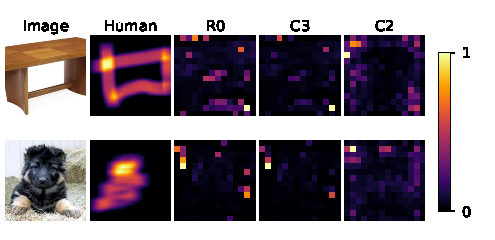
\includegraphics[width=0.62\linewidth]{../../figures/figure_A_2b_layer12.pdf}
\caption{The two ClickMe images of Figure~\ref{fig:read}(b) (drawn with a fixed seed, not selected): image, human map, R0, C3 and C2 of DeiT-S, all at layer 12 alone; each map scaled to $[0,1]$.}
\label{fig:layer12}
\end{figure}

\FloatBarrier
\section{Pre-registration and checks}
\label{app:prereg}

\textbf{What was fixed before the runs.} Before the first main run, a dated entry in the project's decision log (a git commit) fixed the readings, stand-ins, references, data and held-out set, the three metrics and their margins, the statistics, the primary comparisons and predictions P1--P7. One implementation-check tolerance was then raised from $10^{-4}$ to $5\times10^{-4}$ because DeiT-B gave $1.4\times10^{-4}$ (identical classes); no research definition changed. Every exploratory analysis (Appendices~\ref{app:full} and~\ref{app:c2}) was proposed after the main results; its definitions and decision rules were committed before it ran. Some results had been seen before registration: the DeiT-S $k$ sweep, the earlier per-layer curves and probe, and the attention-budget results, so P1 (DeiT-S) and the M2 and M3 parts of P2 are replications.

\textbf{Predictions.} P1: execution agreement rises with $k$, and reading sets beat random sets at every $k$. P2: M2 becomes more severe with depth; M3 concentrates in layers 6--12 of supervised models and is near 0 in DINO. P3 (main verdict): R\_all, the combination C3$\to$C2$\to$C1, is higher than R0 on enrichment and ClickMe in the two supervised models (4 cells; all 4 = holds, 1--3 = partly holds). P4: negative controls (C3 on DINO; C2 at layers 1--4) are comparable to R0; otherwise the runs stop. P5: the share of the last-layer drop that each correction recovers (descriptive). P6: the two model-side variants are not higher than DeiT-S R0. P7: the primary comparisons, with no predicted direction, are R\_all $-$ R0 and each correction minus its stand-in. Table~\ref{tab:predictions} gives the outcomes.

% Generated by make_appendix_tables.py from the CSV files in the results directory; do not edit by hand.
\begin{table}[!htbp]
\centering
\small
\setlength{\tabcolsep}{4pt}
\caption{Registered predictions and their outcomes (decision rules in App.~C). P7 lists the primary comparisons (correction $-$ stand-in, three metrics), for which no direction was predicted (holds = ---). P3 has 1 of 4 cells higher, which its pre-agreed reading scores as ``partly holds''. P5 (last-layer recovery) is descriptive and is reported in Table~\ref{tab:last_layer}.}
\label{tab:predictions}
\begin{tabular}{lllp{7.3cm}}
\toprule
Prediction & Model(s) & Holds & Detail \\
\midrule
P1 & DeiT-S & yes & \raggedright 11/11 tests \tabularnewline
 & DeiT-B & yes & \raggedright 11/11 tests \tabularnewline
 & DINO & yes & \raggedright 11/11 tests \tabularnewline
\addlinespace[2pt]
P2 & DeiT-S & yes & \raggedright M2 deepens: accuracy L12 $<$ L1 and Spearman(layer, accuracy) $\le$ $-$0.8 \tabularnewline
 & DeiT-S & yes & \raggedright M3: largest high-norm share in layers 6--12 \tabularnewline
 & DeiT-B & yes & \raggedright M2 deepens: accuracy L12 $<$ L1 and Spearman(layer, accuracy) $\le$ $-$0.8 \tabularnewline
 & DeiT-B & yes & \raggedright M3: largest high-norm share in layers 6--12 \tabularnewline
 & DINO & yes & \raggedright M2 deepens: accuracy L12 $<$ L1 and Spearman(layer, accuracy) $\le$ $-$0.8 \tabularnewline
 & DINO & yes & \raggedright M3: DINO high-norm share upper bound $<$ 0.01 at every layer \tabularnewline
\addlinespace[2pt]
P3 & DeiT-S, DeiT-B & no & \raggedright 1/4 cells higher; case: partial \tabularnewline
\addlinespace[2pt]
P7 & DeiT-S & --- & \raggedright C1 vs stand-in: enrichment comparable, SRG comparable, ClickMe comparable \tabularnewline
 & DeiT-S & --- & \raggedright C2 vs stand-in: enrichment lower, SRG lower, ClickMe lower \tabularnewline
 & DeiT-S & --- & \raggedright C3 vs stand-in: enrichment higher, SRG comparable, ClickMe higher \tabularnewline
 & DeiT-B & --- & \raggedright C1 vs stand-in: enrichment higher, SRG higher, ClickMe higher \tabularnewline
 & DeiT-B & --- & \raggedright C2 vs stand-in: enrichment higher, SRG comparable, ClickMe comparable \tabularnewline
 & DeiT-B & --- & \raggedright C3 vs stand-in: enrichment higher, SRG comparable, ClickMe comparable \tabularnewline
 & DINO & --- & \raggedright C1 vs stand-in: enrichment comparable, SRG comparable, ClickMe comparable \tabularnewline
 & DINO & --- & \raggedright C2 vs stand-in: enrichment lower, SRG lower, ClickMe lower \tabularnewline
 & DINO & --- & \raggedright C3 vs stand-in: enrichment comparable, SRG comparable, ClickMe comparable \tabularnewline
\addlinespace[2pt]
P4a & DINO & yes & \raggedright 3/3 comparable \tabularnewline
\addlinespace[2pt]
P4b & DeiT-S, DeiT-B, DINO & yes & \raggedright 6/6 comparable \tabularnewline
\addlinespace[2pt]
P6 & +register, MiTA-DeiT-S & yes & \raggedright 4/4 not higher \tabularnewline
\bottomrule
\end{tabular}
\end{table}


\textbf{Negative controls and reproduction check.} Both negative controls are comparable in every cell, and the new R0 reproduces the earlier full-attention runs on the same images (all differences below the registered 0.01; Table~\ref{tab:controls}).

% Generated by make_appendix_tables.py from the CSV files in the results directory; do not edit by hand.
\begin{table}[!htbp]
\centering
\small
\setlength{\tabcolsep}{4pt}
\caption{Checks. (a) Pre-registered negative controls (P4): P4a = C3 $-$ R0 on DINO (layers 9--12), P4b = C2 $-$ R0 at layers 1--4; differences (4 decimals) with 95\% paired-bootstrap intervals and verdicts (margin 0.05 for SRG, 0.02 otherwise); SRG is not used for P4b by design. Data: ImageNet-S (SRG, enrichment) and ClickMe. (b) Reproduction check: mean of the new R0 (layers 9--12) vs the earlier full-attention runs on the same images; registered criterion $|$difference$|$ $< 0.01$.}
\label{tab:controls}
\par\medskip\textit{(a) Negative controls}\par\smallskip
\begin{tabular}{lllrcc}
\toprule
Control & Model & Metric & $n$ & Difference & Verdict \\
\midrule
P4a & DINO & SRG & 2,000 & 0.0003 [$-$0.0032, 0.0039] & comparable \\
P4a & DINO & Enrichment & 12,144 & $-$0.0035 [$-$0.0040, $-$0.0030] & comparable \\
P4a & DINO & ClickMe & 17,408 & $-$0.0007 [$-$0.0010, $-$0.0005] & comparable \\
P4b & DeiT-S & Enrichment & 12,150 & $-$0.0010 [$-$0.0015, $-$0.0005] & comparable \\
P4b & DeiT-S & ClickMe & 17,408 & $-$0.0002 [$-$0.0004, 0.0000] & comparable \\
P4b & DeiT-B & Enrichment & 12,150 & 0.0000 [$-$0.0001, 0.0002] & comparable \\
P4b & DeiT-B & ClickMe & 17,408 & 0.0000 [$-$0.0001, 0.0000] & comparable \\
P4b & DINO & Enrichment & 12,144 & $-$0.0037 [$-$0.0043, $-$0.0030] & comparable \\
P4b & DINO & ClickMe & 17,408 & $-$0.0017 [$-$0.0018, $-$0.0015] & comparable \\
\bottomrule
\end{tabular}
\par\medskip\textit{(b) Reproduction check}\par\smallskip
\begin{tabular}{llrcccc}
\toprule
Model & Metric & $n$ & New R0 & Earlier & Difference ($\times 10^{-3}$) & $< 0.01$ \\
\midrule
DeiT-S & Enrichment & 12,150 & 0.1401 & 0.1400 & 0.056 & yes \\
DeiT-S & SRG & 2,000 & 0.2360 & 0.2357 & 0.326 & yes \\
DeiT-S & ClickMe & 17,408 & 0.1565 & 0.1564 & 0.158 & yes \\
DeiT-B & Enrichment & 12,150 & 0.0805 & 0.0805 & 0.000 & yes \\
DeiT-B & SRG & 2,000 & 0.1694 & 0.1694 & 0.001 & yes \\
DeiT-B & ClickMe & 17,408 & 0.1071 & 0.1071 & 0.000 & yes \\
DINO & Enrichment & 12,144 & 0.1994 & 0.1994 & $-$0.012 & yes \\
DINO & SRG & 2,000 & 0.2850 & 0.2852 & $-$0.188 & yes \\
DINO & ClickMe & 17,408 & 0.2076 & 0.2078 & $-$0.143 & yes \\
\bottomrule
\end{tabular}
\end{table}


\textbf{Model-randomisation sanity check.} We re-initialise the model cumulatively, one stage at a time from the classifier down to the patch embedding, \citep{adebayo2018} on 1,000 ImageNet-S images and report the median Spearman correlation between the map of the randomised model and the original map. A reading passes if this median is below 0.5 after full randomisation. All readings pass (largest median 0.37); the centred Gaussian does not depend on the model and serves as the example that fails (Table~\ref{tab:sanity}).

% Generated by make_appendix_tables.py from the CSV files in the results directory; do not edit by hand.
\begin{table}[!htbp]
\centering
\small
\setlength{\tabcolsep}{4pt}
\caption{Model-randomisation sanity check on 1,000 ImageNet-S images: median per-image Spearman correlation between the map of the fully randomised model (all stages re-initialised down to the patch embedding) and the map of the trained model (layers 9--12). A reading passes if the median is below 0.5. The centre Gaussian does not depend on the model and is the designed failing example.}
\label{tab:sanity}
\begin{tabular}{lcccccc}
\toprule
 & \multicolumn{2}{c}{DeiT-S} & \multicolumn{2}{c}{DeiT-B} & \multicolumn{2}{c}{DINO} \\
\cmidrule(lr){2-3} \cmidrule(lr){4-5} \cmidrule(lr){6-7}
Reading & median & & median & & median & \\
\midrule
R0 & $-$0.033 & passes & 0.055 & passes & 0.071 & passes \\
C1 & 0.187 & passes & 0.366 & passes & 0.100 & passes \\
C2 & 0.063 & passes & 0.004 & passes & $-$0.002 & passes \\
C3 & $-$0.064 & passes & 0.070 & passes & 0.114 & passes \\
$R_{\mathrm{all}}$ (C3$\to$C2$\to$C1) & 0.069 & passes & 0.078 & passes & 0.025 & passes \\
\midrule
Centre Gaussian (reference) & 1.000 & fails & 1.000 & fails & 1.000 & fails \\
\bottomrule
\end{tabular}
\end{table}


\FloatBarrier
\section{Full Table 1 and exploratory checks of C3}
\label{app:full}

Tables~\ref{tab:full_srg}--\ref{tab:full_clickme} give every reading, stand-in and reference on all three metrics with intervals; SRG uses the fixed 2,000 ImageNet-S images. Table~\ref{tab:diffs} gives the paired differences with their verdicts, Table~\ref{tab:variants} the model-side variants, Table~\ref{tab:order} the two orders of combining all three corrections and Table~\ref{tab:last_layer} the share of the last-layer drop that each correction recovers.

% Generated by make_appendix_tables.py from the CSV files in the results directory; do not edit by hand.
\begin{table}[!htbp]
\centering
\small
\setlength{\tabcolsep}{3pt}
\caption{Full Table~1, deletion faithfulness (SRG) (layers 9--12; higher is better), 2,000 ImageNet-S images, $n$ = 2,000 per model. Mean over images with 95\% bootstrap interval (1,000 resamples over images). Each correction is followed by its stand-in ($\llcorner$). GAE uses gradients and the class and is a reference, not a competitor. SRG is not defined for MiTA, whose summary slots pool fixed regions of the full grid (App.~A).}
\label{tab:full_srg}
\begin{tabular}{lccc}
\toprule
Reading & DeiT-S & DeiT-B & DINO \\
\midrule
R0 (attention received) & 0.236 [0.226, 0.246] & 0.169 [0.160, 0.178] & 0.285 [0.273, 0.296] \\
C3 contribution weighting & 0.253 [0.242, 0.263] & 0.198 [0.188, 0.208] & 0.285 [0.274, 0.296] \\
\hspace{0.6em}$\llcorner$ zero high-norm tokens & 0.241 [0.230, 0.251] & 0.186 [0.176, 0.195] & 0.285 [0.273, 0.296] \\
C2 relocation by probe & 0.076 [0.066, 0.084] & 0.051 [0.044, 0.059] & 0.141 [0.131, 0.151] \\
\hspace{0.6em}$\llcorner$ matched blur & 0.181 [0.170, 0.191] & 0.097 [0.088, 0.107] & 0.287 [0.275, 0.299] \\
C1 subtract mean map & 0.208 [0.197, 0.217] & 0.144 [0.135, 0.153] & 0.233 [0.221, 0.245] \\
\hspace{0.6em}$\llcorner$ subtract centre Gaussian & 0.167 [0.156, 0.177] & 0.024 [0.015, 0.033] & 0.232 [0.220, 0.244] \\
$R_{\mathrm{all}}$ (C3$\to$C2$\to$C1) & 0.076 [0.067, 0.085] & 0.085 [0.077, 0.093] & 0.090 [0.080, 0.100] \\
Other order (C3$\to$C1$\to$C2) & 0.168 [0.157, 0.178] & 0.159 [0.150, 0.170] & 0.223 [0.211, 0.234] \\
\midrule
\multicolumn{4}{l}{\textit{References}} \\
Random & $-$0.002 [$-$0.009, 0.005] & $-$0.003 [$-$0.009, 0.004] & $-$0.002 [$-$0.009, 0.005] \\
Centre Gaussian & 0.110 [0.100, 0.120] & 0.099 [0.089, 0.109] & 0.140 [0.129, 0.151] \\
Mean map & 0.058 [0.048, 0.068] & 0.011 [0.004, 0.017] & 0.139 [0.128, 0.150] \\
GAE & 0.345 [0.334, 0.355] & 0.308 [0.297, 0.319] & 0.418 [0.406, 0.428] \\
\midrule
\multicolumn{4}{l}{\textit{Change the model (DeiT-S)}} \\
+ test-time register & 0.236 [0.225, 0.246] & --- & --- \\
top-$k$ training (MiTA) & n/a & --- & --- \\
\bottomrule
\end{tabular}
\end{table}

% Generated by make_appendix_tables.py from the CSV files in the results directory; do not edit by hand.
\begin{table}[!htbp]
\centering
\small
\setlength{\tabcolsep}{3pt}
\caption{Full Table~1, same-ring object enrichment (layers 9--12; higher is better), ImageNet-S, $n$ = 12,150 (DeiT-S, DeiT-B) and 12,144 (DINO) per model. Mean over images with 95\% bootstrap interval (1,000 resamples over images). Each correction is followed by its stand-in ($\llcorner$). GAE uses gradients and the class and is a reference, not a competitor. MiTA: $n$ = 12,144 (own crop 0.875).}
\label{tab:full_enrichment}
\begin{tabular}{lccc}
\toprule
Reading & DeiT-S & DeiT-B & DINO \\
\midrule
R0 (attention received) & 0.140 [0.138, 0.142] & 0.080 [0.079, 0.082] & 0.199 [0.196, 0.203] \\
C3 contribution weighting & 0.178 [0.175, 0.180] & 0.146 [0.143, 0.149] & 0.196 [0.193, 0.199] \\
\hspace{0.6em}$\llcorner$ zero high-norm tokens & 0.152 [0.149, 0.154] & 0.121 [0.118, 0.123] & 0.199 [0.196, 0.203] \\
C2 relocation by probe & 0.041 [0.040, 0.043] & 0.027 [0.026, 0.028] & 0.084 [0.083, 0.086] \\
\hspace{0.6em}$\llcorner$ matched blur & 0.095 [0.092, 0.098] & $-$0.008 [$-$0.010, $-$0.007] & 0.189 [0.186, 0.193] \\
C1 subtract mean map & 0.138 [0.136, 0.140] & 0.077 [0.076, 0.079] & 0.201 [0.198, 0.204] \\
\hspace{0.6em}$\llcorner$ subtract centre Gaussian & 0.133 [0.131, 0.135] & 0.056 [0.054, 0.057] & 0.200 [0.197, 0.203] \\
$R_{\mathrm{all}}$ (C3$\to$C2$\to$C1) & 0.059 [0.057, 0.061] & 0.079 [0.077, 0.081] & 0.088 [0.086, 0.090] \\
Other order (C3$\to$C1$\to$C2) & 0.108 [0.106, 0.110] & 0.123 [0.120, 0.125] & 0.156 [0.153, 0.158] \\
\midrule
\multicolumn{4}{l}{\textit{References}} \\
Random & 0.000 [$-$0.001, 0.001] & 0.000 [$-$0.001, 0.001] & 0.000 [$-$0.001, 0.001] \\
Centre Gaussian & 0.000 [0.000, 0.000] & 0.000 [0.000, 0.000] & 0.000 [0.000, 0.000] \\
Mean map & $-$0.003 [$-$0.004, $-$0.003] & $-$0.002 [$-$0.003, $-$0.002] & 0.003 [0.002, 0.003] \\
GAE & 0.204 [0.200, 0.207] & 0.196 [0.193, 0.199] & 0.221 [0.218, 0.225] \\
\midrule
\multicolumn{4}{l}{\textit{Change the model (DeiT-S)}} \\
+ test-time register & 0.152 [0.150, 0.155] & --- & --- \\
top-$k$ training (MiTA) & 0.100 [0.098, 0.102] & --- & --- \\
\bottomrule
\end{tabular}
\end{table}

% Generated by make_appendix_tables.py from the CSV files in the results directory; do not edit by hand.
\begin{table}[!htbp]
\centering
\small
\setlength{\tabcolsep}{3pt}
\caption{Full Table~1, image-specific ClickMe alignment (layers 9--12; higher is better), ClickMe, $n$ = 17,408 per model. Mean over images with 95\% bootstrap interval (1,000 resamples over images). Each correction is followed by its stand-in ($\llcorner$). GAE uses gradients and the class and is a reference, not a competitor.}
\label{tab:full_clickme}
\begin{tabular}{lccc}
\toprule
Reading & DeiT-S & DeiT-B & DINO \\
\midrule
R0 (attention received) & 0.157 [0.154, 0.160] & 0.107 [0.104, 0.110] & 0.208 [0.203, 0.212] \\
C3 contribution weighting & 0.190 [0.186, 0.193] & 0.165 [0.162, 0.168] & 0.207 [0.202, 0.211] \\
\hspace{0.6em}$\llcorner$ zero high-norm tokens & 0.168 [0.165, 0.171] & 0.148 [0.145, 0.151] & 0.208 [0.203, 0.212] \\
C2 relocation by probe & 0.084 [0.080, 0.087] & 0.050 [0.047, 0.053] & 0.143 [0.140, 0.147] \\
\hspace{0.6em}$\llcorner$ matched blur & 0.152 [0.147, 0.157] & 0.068 [0.064, 0.072] & 0.226 [0.221, 0.231] \\
C1 subtract mean map & 0.165 [0.162, 0.169] & 0.087 [0.084, 0.090] & 0.252 [0.247, 0.256] \\
\hspace{0.6em}$\llcorner$ subtract centre Gaussian & 0.168 [0.165, 0.172] & 0.062 [0.058, 0.067] & 0.253 [0.248, 0.257] \\
$R_{\mathrm{all}}$ (C3$\to$C2$\to$C1) & 0.123 [0.119, 0.127] & 0.137 [0.134, 0.140] & 0.177 [0.173, 0.180] \\
Other order (C3$\to$C1$\to$C2) & 0.221 [0.217, 0.225] & 0.199 [0.196, 0.203] & 0.263 [0.258, 0.267] \\
\midrule
\multicolumn{4}{l}{\textit{References}} \\
Random & 0.000 [$-$0.001, 0.002] & 0.000 [$-$0.001, 0.002] & 0.000 [$-$0.001, 0.002] \\
Centre Gaussian & 0.000 [$-$0.005, 0.005] & 0.000 [$-$0.005, 0.005] & 0.000 [$-$0.005, 0.005] \\
Mean map & 0.000 [$-$0.004, 0.004] & 0.000 [$-$0.002, 0.002] & 0.000 [$-$0.005, 0.005] \\
GAE & 0.234 [0.230, 0.238] & 0.213 [0.209, 0.218] & 0.234 [0.230, 0.239] \\
\midrule
\multicolumn{4}{l}{\textit{Change the model (DeiT-S)}} \\
+ test-time register & 0.169 [0.166, 0.173] & --- & --- \\
top-$k$ training (MiTA) & 0.115 [0.112, 0.118] & --- & --- \\
\bottomrule
\end{tabular}
\end{table}

% Generated by make_appendix_tables.py from the CSV files in the results directory; do not edit by hand.
\begin{table}[!htbp]
\centering
\footnotesize
\setlength{\tabcolsep}{3pt}
\caption{Paired differences, layers 9--12: mean with 95\% paired-bootstrap interval and verdict. Verdicts: \textit{h} = higher, \textit{c} = comparable, \textit{l} = lower (interval excludes 0 and $|$difference$|$ exceeds the margin, 0.05 for SRG and 0.02 otherwise). $^\dagger$ = pre-registered primary comparison. centre sub.\ = subtract centre Gaussian; blur = matched blur; zero h.n.\ = zero high-norm tokens. SRG: 2,000 ImageNet-S images; enrichment: ImageNet-S; ClickMe: 17,408 images.}
\label{tab:diffs}
\begin{tabular}{lccc}
\toprule
Comparison & SRG & Enrichment & ClickMe \\
\midrule
\multicolumn{4}{l}{\textit{DeiT-S}} \\
C1 $-$ R0 & $-$0.028 [$-$0.034, $-$0.023]\,\textit{c} & $-$0.002 [$-$0.003, $-$0.002]\,\textit{c} & 0.009 [0.008, 0.010]\,\textit{c} \\
C2 $-$ R0 & $-$0.161 [$-$0.171, $-$0.150]\,\textit{l} & $-$0.099 [$-$0.101, $-$0.097]\,\textit{l} & $-$0.073 [$-$0.076, $-$0.069]\,\textit{l} \\
C3 $-$ R0 & 0.017 [0.013, 0.021]\,\textit{c} & 0.038 [0.036, 0.039]\,\textit{h} & 0.033 [0.032, 0.034]\,\textit{h} \\
$R_{\mathrm{all}}$ $-$ R0$^\dagger$ & $-$0.160 [$-$0.171, $-$0.149]\,\textit{l} & $-$0.081 [$-$0.083, $-$0.079]\,\textit{l} & $-$0.034 [$-$0.038, $-$0.030]\,\textit{l} \\
C1 $-$ centre sub.$^\dagger$ & 0.040 [0.034, 0.047]\,\textit{c} & 0.005 [0.004, 0.005]\,\textit{c} & $-$0.003 [$-$0.005, $-$0.001]\,\textit{c} \\
C2 $-$ blur$^\dagger$ & $-$0.105 [$-$0.116, $-$0.095]\,\textit{l} & $-$0.054 [$-$0.056, $-$0.051]\,\textit{l} & $-$0.068 [$-$0.073, $-$0.064]\,\textit{l} \\
C3 $-$ zero h.n.$^\dagger$ & 0.012 [0.008, 0.016]\,\textit{c} & 0.026 [0.025, 0.027]\,\textit{h} & 0.022 [0.021, 0.023]\,\textit{h} \\
centre sub. $-$ R0 & $-$0.069 [$-$0.076, $-$0.062]\,\textit{l} & $-$0.007 [$-$0.008, $-$0.007]\,\textit{c} & 0.012 [0.009, 0.015]\,\textit{c} \\
blur $-$ R0 & $-$0.055 [$-$0.064, $-$0.046]\,\textit{l} & $-$0.045 [$-$0.047, $-$0.043]\,\textit{l} & $-$0.005 [$-$0.008, $-$0.001]\,\textit{c} \\
zero h.n. $-$ R0 & 0.005 [0.002, 0.008]\,\textit{c} & 0.012 [0.011, 0.013]\,\textit{c} & 0.011 [0.011, 0.012]\,\textit{c} \\
\midrule
\multicolumn{4}{l}{\textit{DeiT-B}} \\
C1 $-$ R0 & $-$0.025 [$-$0.031, $-$0.019]\,\textit{c} & $-$0.003 [$-$0.004, $-$0.003]\,\textit{c} & $-$0.020 [$-$0.021, $-$0.019]\,\textit{l} \\
C2 $-$ R0 & $-$0.118 [$-$0.127, $-$0.110]\,\textit{l} & $-$0.054 [$-$0.055, $-$0.052]\,\textit{l} & $-$0.057 [$-$0.059, $-$0.055]\,\textit{l} \\
C3 $-$ R0 & 0.029 [0.024, 0.034]\,\textit{c} & 0.065 [0.063, 0.067]\,\textit{h} & 0.058 [0.056, 0.059]\,\textit{h} \\
$R_{\mathrm{all}}$ $-$ R0$^\dagger$ & $-$0.084 [$-$0.093, $-$0.076]\,\textit{l} & $-$0.001 [$-$0.003, 0.001]\,\textit{c} & 0.030 [0.027, 0.032]\,\textit{h} \\
C1 $-$ centre sub.$^\dagger$ & 0.120 [0.109, 0.130]\,\textit{h} & 0.022 [0.021, 0.023]\,\textit{h} & 0.025 [0.020, 0.030]\,\textit{h} \\
C2 $-$ blur$^\dagger$ & $-$0.047 [$-$0.055, $-$0.037]\,\textit{c} & 0.035 [0.034, 0.036]\,\textit{h} & $-$0.018 [$-$0.020, $-$0.015]\,\textit{c} \\
C3 $-$ zero h.n.$^\dagger$ & 0.013 [0.008, 0.018]\,\textit{c} & 0.025 [0.024, 0.026]\,\textit{h} & 0.017 [0.016, 0.018]\,\textit{c} \\
centre sub. $-$ R0 & $-$0.146 [$-$0.156, $-$0.135]\,\textit{l} & $-$0.025 [$-$0.026, $-$0.024]\,\textit{l} & $-$0.045 [$-$0.050, $-$0.040]\,\textit{l} \\
blur $-$ R0 & $-$0.072 [$-$0.080, $-$0.064]\,\textit{l} & $-$0.089 [$-$0.091, $-$0.087]\,\textit{l} & $-$0.039 [$-$0.042, $-$0.036]\,\textit{l} \\
zero h.n. $-$ R0 & 0.016 [0.012, 0.020]\,\textit{c} & 0.040 [0.038, 0.042]\,\textit{h} & 0.041 [0.039, 0.042]\,\textit{h} \\
\midrule
\multicolumn{4}{l}{\textit{DINO}} \\
C1 $-$ R0 & $-$0.052 [$-$0.059, $-$0.044]\,\textit{l} & 0.002 [0.001, 0.003]\,\textit{c} & 0.044 [0.040, 0.048]\,\textit{h} \\
C2 $-$ R0 & $-$0.144 [$-$0.153, $-$0.134]\,\textit{l} & $-$0.115 [$-$0.117, $-$0.113]\,\textit{l} & $-$0.064 [$-$0.067, $-$0.062]\,\textit{l} \\
C3 $-$ R0 & 0.000 [$-$0.003, 0.004]\,\textit{c} & $-$0.004 [$-$0.004, $-$0.003]\,\textit{c} & $-$0.001 [$-$0.001, $-$0.001]\,\textit{c} \\
$R_{\mathrm{all}}$ $-$ R0$^\dagger$ & $-$0.195 [$-$0.205, $-$0.184]\,\textit{l} & $-$0.111 [$-$0.114, $-$0.109]\,\textit{l} & $-$0.031 [$-$0.035, $-$0.027]\,\textit{l} \\
C1 $-$ centre sub.$^\dagger$ & 0.001 [$-$0.003, 0.005]\,\textit{c} & 0.001 [0.001, 0.002]\,\textit{c} & $-$0.001 [$-$0.001, 0.000]\,\textit{c} \\
C2 $-$ blur$^\dagger$ & $-$0.146 [$-$0.155, $-$0.137]\,\textit{l} & $-$0.105 [$-$0.107, $-$0.102]\,\textit{l} & $-$0.083 [$-$0.085, $-$0.080]\,\textit{l} \\
C3 $-$ zero h.n.$^\dagger$ & 0.000 [$-$0.003, 0.004]\,\textit{c} & $-$0.004 [$-$0.004, $-$0.003]\,\textit{c} & $-$0.001 [$-$0.001, $-$0.001]\,\textit{c} \\
centre sub. $-$ R0 & $-$0.053 [$-$0.060, $-$0.045]\,\textit{l} & 0.001 [0.000, 0.001]\,\textit{c} & 0.045 [0.041, 0.048]\,\textit{h} \\
blur $-$ R0 & 0.002 [$-$0.005, 0.009]\,\textit{c} & $-$0.010 [$-$0.012, $-$0.009]\,\textit{c} & 0.018 [0.017, 0.019]\,\textit{c} \\
zero h.n. $-$ R0 & 0.000 [0.000, 0.000]\,\textit{c} & 0.000 [0.000, 0.000]\,\textit{c} & 0.000 [0.000, 0.000]\,\textit{c} \\
\bottomrule
\end{tabular}
\end{table}

% Generated by make_appendix_tables.py from the CSV files in the results directory; do not edit by hand.
\begin{table}[!htbp]
\centering
\small
\setlength{\tabcolsep}{3.5pt}
\caption{Changing the model (DeiT-S, layers 9--12): R0 of DeiT-S with a test-time register and of MiTA-DeiT-S (top-$k$ training), paired with DeiT-S R0 by image index; mean difference with 95\% paired-bootstrap interval, verdict, and the registered check P6 (2) (not higher on enrichment and ClickMe). MiTA has no SRG (App.~A) and uses its own crop. Last rows: C3 $-$ R0 on DeiT-S for comparison.}
\label{tab:variants}
\begin{tabular}{llrcccc}
\toprule
Row & Metric & $n$ & Value & Difference vs DeiT-S R0 & Verdict & P6 (2) \\
\midrule
+ test-time register & SRG & 2,000 & 0.236 & 0.000 [$-$0.005, 0.004] & comparable & --- \\
+ test-time register & Enrichment & 12,150 & 0.152 & 0.012 [0.011, 0.013] & comparable & not higher \\
+ test-time register & ClickMe & 17,408 & 0.169 & 0.013 [0.012, 0.013] & comparable & not higher \\
\midrule
top-$k$ training (MiTA) & SRG & --- & n/a & n/a &  &  \\
top-$k$ training (MiTA) & Enrichment & 12,118 & 0.100 & $-$0.040 [$-$0.042, $-$0.039] & lower & not higher \\
top-$k$ training (MiTA) & ClickMe & 17,408 & 0.115 & $-$0.042 [$-$0.044, $-$0.040] & lower & not higher \\
\midrule
For comparison: C3 & SRG & 2,000 &  & 0.017 [0.013, 0.021] & comparable &  \\
For comparison: C3 & Enrichment & 12,150 &  & 0.038 [0.036, 0.039] & higher &  \\
For comparison: C3 & ClickMe & 17,408 &  & 0.033 [0.032, 0.034] & higher &  \\
\bottomrule
\end{tabular}
\end{table}

% Generated by make_appendix_tables.py from the CSV files in the results directory; do not edit by hand.
\begin{table}[!htbp]
\centering
\footnotesize
\setlength{\tabcolsep}{3.5pt}
\caption{Combination orders (layers 9--12): $R_{\mathrm{all}}$ = C3$\to$C2$\to$C1 (registered), Other order = C3$\to$C1$\to$C2 (descriptive check). Values (95\% bootstrap intervals $\le \pm$0.012) and paired differences with 95\% paired-bootstrap intervals and verdicts. Verdicts: \textit{h} = higher, \textit{c} = comparable, \textit{l} = lower (interval excludes 0 and $|$difference$|$ exceeds the margin, 0.05 for SRG and 0.02 otherwise). The two orders get the same verdict against R0 in 5 of 9 cells (``robust'' required all 9).}
\label{tab:order}
\begin{tabular}{lccccc}
\toprule
Metric & R0 & $R_{\mathrm{all}}$ & Other order & $R_{\mathrm{all}}$ $-$ R0 & Other order $-$ $R_{\mathrm{all}}$ \\
\midrule
\multicolumn{6}{l}{\textit{DeiT-S}} \\
SRG & 0.236 & 0.076 & 0.168 & $-$0.160 [$-$0.171, $-$0.149]\,\textit{l} & 0.091 [0.082, 0.100]\,\textit{h} \\
Enrichment & 0.140 & 0.059 & 0.108 & $-$0.081 [$-$0.083, $-$0.079]\,\textit{l} & 0.049 [0.048, 0.050]\,\textit{h} \\
ClickMe & 0.157 & 0.123 & 0.221 & $-$0.034 [$-$0.038, $-$0.030]\,\textit{l} & 0.098 [0.094, 0.102]\,\textit{h} \\
\midrule
\multicolumn{6}{l}{\textit{DeiT-B}} \\
SRG & 0.169 & 0.085 & 0.159 & $-$0.084 [$-$0.093, $-$0.076]\,\textit{l} & 0.074 [0.066, 0.083]\,\textit{h} \\
Enrichment & 0.080 & 0.079 & 0.123 & $-$0.001 [$-$0.003, 0.001]\,\textit{c} & 0.043 [0.042, 0.045]\,\textit{h} \\
ClickMe & 0.107 & 0.137 & 0.199 & 0.030 [0.027, 0.032]\,\textit{h} & 0.062 [0.060, 0.065]\,\textit{h} \\
\midrule
\multicolumn{6}{l}{\textit{DINO}} \\
SRG & 0.285 & 0.090 & 0.223 & $-$0.195 [$-$0.205, $-$0.184]\,\textit{l} & 0.133 [0.123, 0.142]\,\textit{h} \\
Enrichment & 0.199 & 0.088 & 0.156 & $-$0.111 [$-$0.114, $-$0.109]\,\textit{l} & 0.068 [0.066, 0.069]\,\textit{h} \\
ClickMe & 0.208 & 0.177 & 0.263 & $-$0.031 [$-$0.035, $-$0.027]\,\textit{l} & 0.086 [0.083, 0.089]\,\textit{h} \\
\bottomrule
\end{tabular}
\end{table}

% Generated by make_appendix_tables.py from the CSV files in the results directory; do not edit by hand.
\begin{table}[!htbp]
\centering
\small
\setlength{\tabcolsep}{4pt}
\caption{Last-layer recovery (P5, descriptive; supervised models). Drop = R0 at the best of layers 8--11 minus R0 at layer 12. Share recovered = (corrected layer-12 map $-$ R0 layer 12) / drop: 1 = full recovery, negative = worse than R0 at layer 12. 95\% paired-bootstrap intervals of the ratio of means. SRG: 2,000 ImageNet-S images; enrichment: ImageNet-S; ClickMe: 17,408 images.}
\label{tab:last_layer}
\begin{tabular}{lccc}
\toprule
 & SRG & Enrichment & ClickMe \\
\midrule
\multicolumn{4}{l}{\textit{DeiT-S}} \\
Best R0 layer (8--11) & layer 10 & layer 11 & layer 9 \\
Drop to layer 12 & 0.049 & 0.038 & 0.086 \\
C3 recovers & 0.078 [0.004, 0.151] & 0.616 [0.588, 0.645] & 0.306 [0.294, 0.317] \\
C1 recovers & $-$0.964 [$-$1.246, $-$0.750] & $-$0.365 [$-$0.394, $-$0.337] & $-$0.120 [$-$0.133, $-$0.107] \\
C2 recovers & $-$3.479 [$-$4.375, $-$2.867] & $-$2.759 [$-$2.943, $-$2.598] & $-$0.979 [$-$1.043, $-$0.919] \\
$R_{\mathrm{all}}$ recovers & $-$3.286 [$-$4.150, $-$2.712] & $-$2.312 [$-$2.478, $-$2.166] & $-$0.673 [$-$0.735, $-$0.617] \\
\midrule
\multicolumn{4}{l}{\textit{DeiT-B}} \\
Best R0 layer (8--11) & layer 10 & layer 11 & layer 10 \\
Drop to layer 12 & 0.081 & 0.088 & 0.116 \\
C3 recovers & 0.290 [0.234, 0.345] & 0.326 [0.311, 0.339] & 0.448 [0.436, 0.461] \\
C1 recovers & $-$0.692 [$-$0.848, $-$0.547] & $-$0.270 [$-$0.284, $-$0.256] & $-$0.359 [$-$0.380, $-$0.339] \\
C2 recovers & $-$1.928 [$-$2.230, $-$1.647] & $-$0.718 [$-$0.750, $-$0.683] & $-$0.787 [$-$0.820, $-$0.755] \\
$R_{\mathrm{all}}$ recovers & $-$1.501 [$-$1.770, $-$1.266] & $-$0.396 [$-$0.425, $-$0.366] & $-$0.353 [$-$0.381, $-$0.325] \\
\bottomrule
\end{tabular}
\end{table}


\textbf{Exploratory checks of C3 (post hoc).} Table~\ref{tab:c3_checks} compares C3 with three variants: weights shuffled among the tokens of a head, the head's mean weight for every token, and $\lVert v_j\rVert$ instead of $\lVert W_O v_j\rVert$. It also gives the dose--response correlation across images (the gain of C3 against R0's share on high-norm tokens) and the share of the R0-to-GAE gap that C3 closes. Table~\ref{tab:dose_layers} gives the gains at single layers, and Table~\ref{tab:pairs} the pairwise combinations of corrections.

% Generated by make_appendix_tables.py from the CSV files in the results directory; do not edit by hand.
\begin{table}[!htbp]
\centering
\footnotesize
\setlength{\tabcolsep}{4pt}
\caption{Exploratory checks of C3 (layers 9--12). (a) Mechanism: C3 against C3 with its weights $\lVert W_O v_j\rVert$ shuffled among the patch tokens of each head (5 seeds), replaced by the head mean, or replaced by $\lVert v_j\rVert$. Verdicts: \textit{h} = higher, \textit{c} = comparable, \textit{l} = lower (interval excludes 0 and $|$difference$|$ exceeds the margin, 0.05 for SRG and 0.02 otherwise). (b) Dose--response: across images, Spearman correlation between the share of R0 on high-norm tokens (dose) and the image's improvement. (c) Share of the gap between R0 and GAE closed by C3, (C3 $-$ R0) / (GAE $-$ R0). All intervals are 95\% (paired) bootstrap intervals over images. Enrichment: ImageNet-S; ClickMe: 17,408 images; SRG: 2,000 ImageNet-S images.}
\label{tab:c3_checks}
\par\medskip\textit{(a) Mechanism}\par\smallskip
\begin{tabular}{llcc}
\toprule
Comparison & Model & Enrichment & ClickMe \\
\midrule
C3 $-$ C3 with shuffled weights & DeiT-S & 0.038 [0.037, 0.040]\,\textit{h} & 0.035 [0.035, 0.036]\,\textit{h} \\
 & DeiT-B & 0.073 [0.071, 0.076]\,\textit{h} & 0.067 [0.065, 0.068]\,\textit{h} \\
 & DINO & $-$0.004 [$-$0.004, $-$0.003]\,\textit{c} & 0.000 [0.000, 0.000]\,\textit{c} \\
C3 $-$ C3 with head-mean weights & DeiT-S & 0.038 [0.037, 0.040]\,\textit{h} & 0.035 [0.034, 0.036]\,\textit{h} \\
 & DeiT-B & 0.073 [0.071, 0.076]\,\textit{h} & 0.066 [0.065, 0.068]\,\textit{h} \\
 & DINO & $-$0.004 [$-$0.005, $-$0.004]\,\textit{c} & 0.000 [0.000, 0.000]\,\textit{c} \\
C3 $-$ C3 with $\lVert v_j\rVert$ weights & DeiT-S & $-$0.010 [$-$0.011, $-$0.009]\,\textit{c} & $-$0.010 [$-$0.011, $-$0.010]\,\textit{c} \\
 & DeiT-B & $-$0.007 [$-$0.007, $-$0.006]\,\textit{c} & $-$0.006 [$-$0.006, $-$0.006]\,\textit{c} \\
 & DINO & 0.000 [$-$0.001, 0.000]\,\textit{c} & $-$0.001 [$-$0.001, $-$0.001]\,\textit{c} \\
\bottomrule
\end{tabular}
\par\medskip\textit{(b) Dose--response}\par\smallskip
\begin{tabular}{lllrcc}
\toprule
Model & Metric & Improvement & $n$ & Mean dose & Spearman(dose, improvement) \\
\midrule
DeiT-S & Enrichment & C3 $-$ R0 & 12,150 & 0.078 & 0.075 [0.057, 0.092] \\
DeiT-S & Enrichment & C3 $-$ zero high-norm & 12,150 & 0.078 & $-$0.035 [$-$0.052, $-$0.018] \\
DeiT-S & ClickMe & C3 $-$ R0 & 17,408 & 0.082 & 0.045 [0.032, 0.060] \\
DeiT-S & ClickMe & C3 $-$ zero high-norm & 17,408 & 0.082 & $-$0.065 [$-$0.079, $-$0.051] \\
DeiT-B & Enrichment & C3 $-$ R0 & 12,150 & 0.289 & 0.132 [0.113, 0.150] \\
DeiT-B & Enrichment & C3 $-$ zero high-norm & 12,150 & 0.289 & $-$0.031 [$-$0.049, $-$0.013] \\
DeiT-B & ClickMe & C3 $-$ R0 & 17,408 & 0.293 & 0.158 [0.143, 0.173] \\
DeiT-B & ClickMe & C3 $-$ zero high-norm & 17,408 & 0.293 & $-$0.028 [$-$0.044, $-$0.014] \\
\bottomrule
\end{tabular}
\par\medskip\textit{(c) Share of the GAE gap closed}\par\smallskip
\begin{tabular}{llrccc}
\toprule
Model & Metric & $n$ & C3 $-$ R0 & GAE $-$ R0 & Share closed \\
\midrule
DeiT-S & SRG & 2,000 & 0.017 & 0.109 & 0.159 [0.123, 0.195] \\
DeiT-S & Enrichment & 12,150 & 0.038 & 0.063 & 0.592 [0.574, 0.611] \\
DeiT-S & ClickMe & 17,408 & 0.033 & 0.077 & 0.430 [0.420, 0.442] \\
DeiT-B & SRG & 2,000 & 0.029 & 0.138 & 0.208 [0.173, 0.242] \\
DeiT-B & Enrichment & 12,150 & 0.065 & 0.115 & 0.567 [0.554, 0.582] \\
DeiT-B & ClickMe & 17,408 & 0.058 & 0.106 & 0.542 [0.532, 0.554] \\
\bottomrule
\end{tabular}
\end{table}

% Generated by make_appendix_tables.py from the CSV files in the results directory; do not edit by hand.
\begin{table}[!htbp]
\centering
\small
\setlength{\tabcolsep}{4pt}
\caption{Per-layer gains (exploratory): gain over R0 of C3 and of zeroing high-norm tokens (zero h.n.) when only that layer is read, and for layers 9--12 summed. Enrichment: ImageNet-S; ClickMe: 17,408 images. 95\% paired-bootstrap intervals have half-width $\le$ 0.003. Verdicts: \textit{h} = higher, \textit{c} = comparable, \textit{l} = lower (interval excludes 0 and $|$difference$|$ exceeds the margin, 0.05 for SRG and 0.02 otherwise).}
\label{tab:dose_layers}
\begin{tabular}{llcccc}
\toprule
 & & \multicolumn{2}{c}{Enrichment} & \multicolumn{2}{c}{ClickMe} \\
\cmidrule(lr){3-4} \cmidrule(lr){5-6}
Model & Layer & C3 $-$ R0 & zero h.n. $-$ R0 & C3 $-$ R0 & zero h.n. $-$ R0 \\
\midrule
DeiT-S & 8 & 0.020\,\textit{h} & 0.022\,\textit{h} & 0.026\,\textit{h} & 0.027\,\textit{h} \\
 & 9 & 0.031\,\textit{h} & 0.022\,\textit{h} & 0.033\,\textit{h} & 0.024\,\textit{h} \\
 & 10 & 0.038\,\textit{h} & 0.016\,\textit{c} & 0.035\,\textit{h} & 0.018\,\textit{c} \\
 & 11 & 0.046\,\textit{h} & 0.010\,\textit{c} & 0.044\,\textit{h} & 0.009\,\textit{c} \\
 & 12 & 0.023\,\textit{h} & 0.006\,\textit{c} & 0.026\,\textit{h} & 0.007\,\textit{c} \\
 & 9--12 summed & 0.038\,\textit{h} & 0.012\,\textit{c} & 0.033\,\textit{h} & 0.011\,\textit{c} \\
\midrule
DeiT-B & 8 & 0.008\,\textit{c} & 0.030\,\textit{h} & 0.024\,\textit{h} & 0.044\,\textit{h} \\
 & 9 & 0.034\,\textit{h} & 0.041\,\textit{h} & 0.047\,\textit{h} & 0.057\,\textit{h} \\
 & 10 & 0.049\,\textit{h} & 0.055\,\textit{h} & 0.050\,\textit{h} & 0.058\,\textit{h} \\
 & 11 & 0.050\,\textit{h} & 0.055\,\textit{h} & 0.048\,\textit{h} & 0.056\,\textit{h} \\
 & 12 & 0.028\,\textit{h} & 0.014\,\textit{c} & 0.052\,\textit{h} & 0.021\,\textit{h} \\
 & 9--12 summed & 0.065\,\textit{h} & 0.040\,\textit{h} & 0.058\,\textit{h} & 0.041\,\textit{h} \\
\bottomrule
\end{tabular}
\end{table}

% Generated by make_appendix_tables.py from the CSV files in the results directory; do not edit by hand.
\begin{table}[!htbp]
\centering
\footnotesize
\setlength{\tabcolsep}{3pt}
\caption{Pairwise combinations (exploratory), layers 9--12, applied in the order C3$\to$C2$\to$C1 with the absent correction skipped. Paired differences with 95\% paired-bootstrap intervals and verdicts. Verdicts: \textit{h} = higher, \textit{c} = comparable, \textit{l} = lower (interval excludes 0 and $|$difference$|$ exceeds the margin, 0.05 for SRG and 0.02 otherwise). SRG was computed for C1+C3 only (2,000 ImageNet-S images); enrichment: ImageNet-S; ClickMe: 17,408 images.}
\label{tab:pairs}
\begin{tabular}{lccc}
\toprule
Comparison & SRG & Enrichment & ClickMe \\
\midrule
\multicolumn{4}{l}{\textit{DeiT-S}} \\
C1+C3 $-$ R0 & $-$0.019 [$-$0.026, $-$0.013]\,\textit{c} & 0.035 [0.033, 0.036]\,\textit{h} & 0.052 [0.050, 0.054]\,\textit{h} \\
C2+C3 $-$ R0 & --- & $-$0.082 [$-$0.084, $-$0.080]\,\textit{l} & $-$0.045 [$-$0.048, $-$0.041]\,\textit{l} \\
C1+C2 $-$ R0 & --- & $-$0.096 [$-$0.099, $-$0.094]\,\textit{l} & $-$0.066 [$-$0.070, $-$0.062]\,\textit{l} \\
C1+C3 $-$ C3 & $-$0.037 [$-$0.043, $-$0.030]\,\textit{c} & $-$0.003 [$-$0.003, $-$0.002]\,\textit{c} & 0.019 [0.017, 0.021]\,\textit{c} \\
C2+C3 $-$ C3 & --- & $-$0.120 [$-$0.122, $-$0.118]\,\textit{l} & $-$0.078 [$-$0.082, $-$0.075]\,\textit{l} \\
\midrule
\multicolumn{4}{l}{\textit{DeiT-B}} \\
C1+C3 $-$ R0 & 0.001 [$-$0.005, 0.006]\,\textit{c} & 0.065 [0.063, 0.067]\,\textit{h} & 0.074 [0.072, 0.076]\,\textit{h} \\
C2+C3 $-$ R0 & --- & $-$0.002 [$-$0.004, 0.000]\,\textit{c} & 0.021 [0.019, 0.024]\,\textit{h} \\
C1+C2 $-$ R0 & --- & $-$0.051 [$-$0.053, $-$0.050]\,\textit{l} & $-$0.066 [$-$0.068, $-$0.063]\,\textit{l} \\
C1+C3 $-$ C3 & $-$0.028 [$-$0.033, $-$0.023]\,\textit{c} & 0.000 [$-$0.001, 0.000]\,\textit{c} & 0.017 [0.015, 0.019]\,\textit{c} \\
C2+C3 $-$ C3 & --- & $-$0.068 [$-$0.070, $-$0.066]\,\textit{l} & $-$0.036 [$-$0.038, $-$0.034]\,\textit{l} \\
\midrule
\multicolumn{4}{l}{\textit{DINO}} \\
C1+C3 $-$ R0 & $-$0.049 [$-$0.058, $-$0.042]\,\textit{c} & $-$0.002 [$-$0.003, $-$0.001]\,\textit{c} & 0.043 [0.040, 0.047]\,\textit{h} \\
C2+C3 $-$ R0 & --- & $-$0.113 [$-$0.116, $-$0.111]\,\textit{l} & $-$0.061 [$-$0.063, $-$0.059]\,\textit{l} \\
C1+C2 $-$ R0 & --- & $-$0.114 [$-$0.116, $-$0.112]\,\textit{l} & $-$0.037 [$-$0.041, $-$0.034]\,\textit{l} \\
C1+C3 $-$ C3 & $-$0.050 [$-$0.058, $-$0.042]\,\textit{c} & 0.002 [0.001, 0.003]\,\textit{c} & 0.044 [0.040, 0.047]\,\textit{h} \\
C2+C3 $-$ C3 & --- & $-$0.110 [$-$0.112, $-$0.108]\,\textit{l} & $-$0.060 [$-$0.062, $-$0.058]\,\textit{l} \\
\bottomrule
\end{tabular}
\end{table}


\FloatBarrier
\section{Exploratory analysis of C2}
\label{app:c2}

All analyses in this appendix were proposed after the main results; their definitions and decision rules were committed before they ran.

\textbf{Probe errors and probe prior.} For every patch token of the 2,000 held-out test images, $P$ is the probe's distribution over the 196 positions and $j$ the true position (grid distance in patches). Table~\ref{tab:probe_errors} and Figure~\ref{fig:c2}(a, b) give the probe's exact and top-5 accuracy, its probability within the $3\times3$ neighbourhood of $j$, the share of its error mass farther than 3 patches, and its expected distance, compared with the matched blur. The registered hypothesis ``the errors are mostly far'' required a far share above 0.5; the far share is 0.02--0.29 at layers 9--12. The probe's mean prediction over images (Figure~\ref{fig:c2}(c, d)) is close to uniform; the hypothesis that it carries an image-independent position preference was met in none of the 12 model--layer cells.

\begin{figure}[!htbp]
\centering
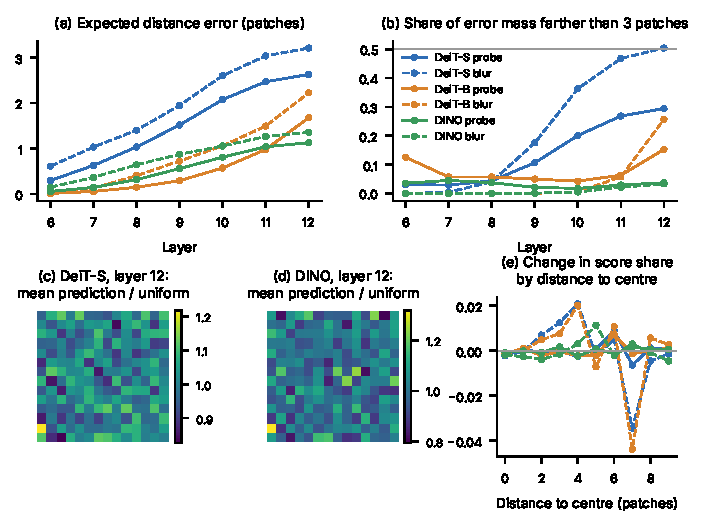
\includegraphics[width=\linewidth]{figure_A_c2.pdf}
\caption{Why C2 fails (exploratory). (a) Expected distance between the true patch and the probe's distribution (solid) or the matched blur (dashed). (b) Share of the error mass farther than 3 patches; the grey line marks the registered threshold 0.5. (c, d) The probe's mean prediction at layer 12 divided by the uniform value $1/196$. (e) Change in the share of the score at each distance from the centre caused by C2 (solid) and by the matched blur (dashed), layers 9--12, ImageNet-S.}
\label{fig:c2}
\end{figure}

% Generated by make_appendix_tables.py from the CSV files in the results directory; do not edit by hand.
\begin{table}[!htbp]
\centering
\small
\setlength{\tabcolsep}{4pt}
\caption{Position-probe errors, layers 9--12 (exploratory; all patch tokens of the 2,000 held-out test images). (a) Exact and top-5 accuracy; probability within the 3$\times$3 neighbourhood of the true patch; far share of errors = probability more than 3 patches away / probability off the true patch; expected distance (patches). Pairs give probe / matched blur (exact and top-5 of the blur are 1 by construction). 95\% bootstrap intervals of the probe values have half-width $\le$ 0.020. (b) The probe's mean prediction over all tokens: its peak divided by the uniform value 1/196, and its Pearson correlation with the model's R0 mean map of that layer, with 95\% bootstrap intervals (images resampled; the point estimate is not a mean over images and can lie outside its interval).}
\label{tab:probe_errors}
\par\medskip\textit{(a) Error geometry}\par\smallskip
\begin{tabular}{llccccc}
\toprule
Model & Layer & Exact & Top-5 & $P$(3$\times$3) & Far share of errors & Expected distance \\
\midrule
DeiT-S & 9 & 0.310 & 0.762 & 0.687 / 0.452 & 0.106 / 0.175 & 1.517 / 1.950 \\
 & 10 & 0.231 & 0.631 & 0.553 / 0.295 & 0.201 / 0.363 & 2.075 / 2.602 \\
 & 11 & 0.194 & 0.556 & 0.478 / 0.231 & 0.268 / 0.468 & 2.469 / 3.037 \\
 & 12 & 0.181 & 0.531 & 0.452 / 0.211 & 0.294 / 0.504 & 2.629 / 3.209 \\
\midrule
DeiT-B & 9 & 0.836 & 0.996 & 0.981 / 0.971 & 0.050 / 0.000 & 0.294 / 0.726 \\
 & 10 & 0.668 & 0.973 & 0.943 / 0.849 & 0.043 / 0.005 & 0.573 / 1.060 \\
 & 11 & 0.492 & 0.891 & 0.845 / 0.631 & 0.063 / 0.058 & 0.981 / 1.494 \\
 & 12 & 0.318 & 0.716 & 0.657 / 0.374 & 0.152 / 0.257 & 1.676 / 2.224 \\
\midrule
DINO & 9 & 0.674 & 0.989 & 0.967 / 0.929 & 0.021 / 0.001 & 0.561 / 0.875 \\
 & 10 & 0.505 & 0.950 & 0.912 / 0.851 & 0.017 / 0.005 & 0.810 / 1.057 \\
 & 11 & 0.392 & 0.881 & 0.837 / 0.745 & 0.029 / 0.021 & 1.039 / 1.265 \\
 & 12 & 0.357 & 0.851 & 0.805 / 0.699 & 0.037 / 0.033 & 1.128 / 1.355 \\
\bottomrule
\end{tabular}
\par\medskip\textit{(b) Mean prediction}\par\smallskip
\begin{tabular}{llcc}
\toprule
Model & Layer & Peak / uniform & Pearson with mean map \\
\midrule
DeiT-S & 9 & 1.222 [1.194, 1.258] & $-$0.047 [$-$0.089, $-$0.002] \\
 & 10 & 1.196 [1.187, 1.238] & $-$0.081 [$-$0.128, $-$0.031] \\
 & 11 & 1.208 [1.178, 1.248] & $-$0.167 [$-$0.215, $-$0.110] \\
 & 12 & 1.218 [1.173, 1.264] & $-$0.179 [$-$0.218, $-$0.129] \\
\midrule
DeiT-B & 9 & 1.136 [1.114, 1.158] & 0.086 [0.045, 0.120] \\
 & 10 & 1.154 [1.132, 1.192] & 0.052 [0.007, 0.093] \\
 & 11 & 1.171 [1.156, 1.218] & 0.004 [$-$0.041, 0.048] \\
 & 12 & 1.190 [1.187, 1.269] & 0.052 [$-$0.006, 0.106] \\
\midrule
DINO & 9 & 1.245 [1.222, 1.271] & $-$0.012 [$-$0.038, 0.011] \\
 & 10 & 1.309 [1.280, 1.339] & $-$0.027 [$-$0.059, 0.006] \\
 & 11 & 1.334 [1.301, 1.367] & $-$0.037 [$-$0.074, 0.000] \\
 & 12 & 1.317 [1.283, 1.353] & $-$0.035 [$-$0.073, 0.003] \\
\bottomrule
\end{tabular}
\end{table}


\textbf{Where C2 moves the score.} Table~\ref{tab:shift} compares how much score C2 and the matched blur move off the object, and how they change the ranking of patches.

% Generated by make_appendix_tables.py from the CSV files in the results directory; do not edit by hand.
\begin{table}[!htbp]
\centering
\small
\setlength{\tabcolsep}{4pt}
\caption{Where C2 and the matched blur move the score (exploratory; 12,419 ImageNet-S images, layers 9--12). Object share = score on object patches / score on all valid patches; moved to background = object share of R0 $-$ object share after the change. Correlations: per image, (map $-$ R0) against the layer 9--12 mean map or against closeness to the centre, averaged over images. 95\% bootstrap intervals have half-width $\le$ 0.005. $^\ast$Mean paired difference in same-ring enrichment (Table~\ref{tab:diffs}).}
\label{tab:shift}
\begin{tabular}{lcccccc}
\toprule
 & \multicolumn{2}{c}{DeiT-S} & \multicolumn{2}{c}{DeiT-B} & \multicolumn{2}{c}{DINO} \\
\cmidrule(lr){2-3} \cmidrule(lr){4-5} \cmidrule(lr){6-7}
Quantity & C2 & blur & C2 & blur & C2 & blur \\
\midrule
Object share, R0 & 0.453 & 0.453 & 0.360 & 0.360 & 0.511 & 0.511 \\
Object share, after & 0.413 & 0.415 & 0.360 & 0.363 & 0.471 & 0.482 \\
Moved to background & 0.041 & 0.039 & 0.000 & $-$0.002 & 0.040 & 0.029 \\
Pearson(change, mean map) & $-$0.038 & $-$0.177 & $-$0.037 & $-$0.247 & $-$0.004 & $-$0.080 \\
Spearman(change, mean map) & 0.059 & 0.013 & 0.098 & $-$0.049 & $-$0.012 & $-$0.034 \\
Pearson(change, closeness) & $-$0.002 & 0.058 & $-$0.003 & 0.030 & $-$0.007 & $-$0.013 \\
Spearman(change, closeness) & $-$0.031 & 0.107 & $-$0.074 & $-$0.044 & $-$0.015 & 0.065 \\
\midrule
Enrichment change vs R0$^\ast$ & $-$0.099 & $-$0.045 & $-$0.054 & $-$0.089 & $-$0.115 & $-$0.010 \\
\bottomrule
\end{tabular}
\end{table}


\textbf{Within-layer globalisation.} Within each image and layer, tokens are split into five groups by their cosine similarity to the mean of the other patch tokens. The registered rule required, at layers 10--12 and in at least two models, that more global tokens have both lower probe accuracy and higher probe entropy. Entropy falls with globality in all three models; accuracy falls only in DeiT-B; the rule holds in no model (Table~\ref{tab:global}).

% Generated by make_appendix_tables.py from the CSV files in the results directory; do not edit by hand.
\begin{table}[!htbp]
\centering
\footnotesize
\setlength{\tabcolsep}{4pt}
\caption{Within-layer globalisation (exploratory; 2,000 held-out test images, high-norm tokens excluded). Within each image, tokens are split into 5 groups by their cosine similarity with the image's mean token (5 = most global); per image, Spearman correlation of group number with the probe's exact accuracy, the entropy of its prediction and the expected C2 move, averaged over images, with 95\% bootstrap intervals. The registered rule (higher similarity $\to$ lower accuracy and higher entropy in at least 2 models at each of layers 10--12) is not met.}
\label{tab:global}
\begin{tabular}{llccc}
\toprule
Model & Layer & $\rho$(group, accuracy) & $\rho$(group, entropy) & $\rho$(group, C2 move) \\
\midrule
DeiT-S & 10 & 0.008 [0.003, 0.013] & $-$0.078 [$-$0.085, $-$0.071] & $-$0.053 [$-$0.060, $-$0.046] \\
 & 11 & 0.017 [0.012, 0.021] & $-$0.099 [$-$0.106, $-$0.092] & $-$0.087 [$-$0.093, $-$0.080] \\
 & 12 & 0.021 [0.016, 0.025] & $-$0.111 [$-$0.117, $-$0.104] & $-$0.106 [$-$0.113, $-$0.099] \\
\midrule
DeiT-B & 10 & $-$0.034 [$-$0.039, $-$0.029] & $-$0.068 [$-$0.076, $-$0.061] & $-$0.011 [$-$0.018, $-$0.003] \\
 & 11 & $-$0.082 [$-$0.088, $-$0.076] & $-$0.115 [$-$0.122, $-$0.107] & 0.019 [0.012, 0.026] \\
 & 12 & $-$0.160 [$-$0.165, $-$0.155] & $-$0.103 [$-$0.110, $-$0.095] & 0.096 [0.089, 0.103] \\
\midrule
DINO & 10 & 0.053 [0.048, 0.058] & $-$0.074 [$-$0.082, $-$0.066] & $-$0.065 [$-$0.071, $-$0.058] \\
 & 11 & 0.067 [0.062, 0.072] & $-$0.070 [$-$0.078, $-$0.063] & $-$0.072 [$-$0.079, $-$0.065] \\
 & 12 & 0.082 [0.077, 0.086] & $-$0.094 [$-$0.101, $-$0.087] & $-$0.094 [$-$0.100, $-$0.087] \\
\bottomrule
\end{tabular}
\end{table}


\textbf{A two-layer probe, and moving only confident tokens.} A two-layer MLP probe raises layer-12 accuracy by 1.8 / 3.8 / 6.7 points (DeiT-S / DeiT-B / DINO), and C2 with this probe is still lower than R0 in all six cells. Moving only tokens whose top probability is at least 0.5 removes 37\%--94\% of the loss of C2 but does not remove it (Table~\ref{tab:mlp}).

% Generated by make_appendix_tables.py from the CSV files in the results directory; do not edit by hand.
\begin{table}[!htbp]
\centering
\small
\setlength{\tabcolsep}{4pt}
\caption{Probe capacity and C2 variants (exploratory). (a) Exact accuracy of the linear and the two-layer MLP position probe on the 2,000 held-out test images, with 95\% bootstrap intervals. (b) C2 with the MLP probe, and C2 relocating only tokens whose top probe probability is $\ge 0.5$, against R0 (layers 9--12): paired differences with 95\% paired-bootstrap intervals. Verdicts: \textit{h} = higher, \textit{c} = comparable, \textit{l} = lower (interval excludes 0 and $|$difference$|$ exceeds the margin, 0.05 for SRG and 0.02 otherwise). Enrichment: ImageNet-S; ClickMe: 17,408 images.}
\label{tab:mlp}
\par\medskip\textit{(a) Exact accuracy, linear vs MLP probe}\par\smallskip
\begin{tabular}{llccc}
\toprule
Model & Layer & Linear & MLP & MLP $-$ linear \\
\midrule
DeiT-S & 9 & 0.310 [0.308, 0.312] & 0.334 [0.331, 0.336] & 0.024 \\
 & 10 & 0.231 [0.229, 0.234] & 0.256 [0.254, 0.258] & 0.025 \\
 & 11 & 0.194 [0.192, 0.196] & 0.215 [0.213, 0.217] & 0.022 \\
 & 12 & 0.181 [0.179, 0.183] & 0.199 [0.197, 0.201] & 0.018 \\
\midrule
DeiT-B & 9 & 0.836 [0.835, 0.838] & 0.891 [0.890, 0.893] & 0.055 \\
 & 10 & 0.668 [0.666, 0.671] & 0.709 [0.706, 0.711] & 0.040 \\
 & 11 & 0.492 [0.489, 0.494] & 0.518 [0.515, 0.521] & 0.027 \\
 & 12 & 0.318 [0.315, 0.320] & 0.356 [0.353, 0.359] & 0.038 \\
\midrule
DINO & 9 & 0.674 [0.671, 0.677] & 0.797 [0.794, 0.800] & 0.123 \\
 & 10 & 0.505 [0.502, 0.508] & 0.620 [0.617, 0.623] & 0.115 \\
 & 11 & 0.392 [0.390, 0.395] & 0.477 [0.474, 0.480] & 0.085 \\
 & 12 & 0.357 [0.355, 0.360] & 0.425 [0.422, 0.427] & 0.067 \\
\bottomrule
\end{tabular}
\par\medskip\textit{(b) C2 variants}\par\smallskip
\begin{tabular}{llcc}
\toprule
Comparison & Model & Enrichment & ClickMe \\
\midrule
C2 with MLP probe $-$ R0 & DeiT-S & $-$0.105 [$-$0.107, $-$0.103]\,\textit{l} & $-$0.083 [$-$0.086, $-$0.080]\,\textit{l} \\
 & DeiT-B & $-$0.046 [$-$0.047, $-$0.045]\,\textit{l} & $-$0.048 [$-$0.050, $-$0.047]\,\textit{l} \\
 & DINO & $-$0.097 [$-$0.099, $-$0.094]\,\textit{l} & $-$0.049 [$-$0.050, $-$0.047]\,\textit{l} \\
C2 confident tokens only $-$ R0 & DeiT-S & $-$0.008 [$-$0.009, $-$0.008]\,\textit{c} & $-$0.004 [$-$0.005, $-$0.004]\,\textit{c} \\
 & DeiT-B & $-$0.034 [$-$0.035, $-$0.033]\,\textit{l} & $-$0.025 [$-$0.026, $-$0.024]\,\textit{l} \\
 & DINO & $-$0.040 [$-$0.041, $-$0.038]\,\textit{l} & $-$0.018 [$-$0.019, $-$0.017]\,\textit{c} \\
\bottomrule
\end{tabular}
\end{table}


\textbf{Discounting without relocation.} D2 keeps every score in place and multiplies it by the probe's probability that the unit is still at its own patch; its stand-in shuffles these probabilities among the tokens of the image. Table~\ref{tab:d2} gives the values and tests.

% Generated by make_appendix_tables.py from the CSV files in the results directory; do not edit by hand.
\begin{table}[!htbp]
\centering
\small
\setlength{\tabcolsep}{4pt}
\caption{Discount without relocation (exploratory, layers 9--12). D2 keeps each unit's R0 score at its patch and multiplies it by the probe's probability that the unit is still there; D2 shuffled uses the same probabilities permuted among the tokens of the image and layer (5 seeds); C3D2 applies C3 first. (a) Means (95\% bootstrap intervals $\le \pm$0.005). (b) Paired differences with 95\% paired-bootstrap intervals. Verdicts: \textit{h} = higher, \textit{c} = comparable, \textit{l} = lower (interval excludes 0 and $|$difference$|$ exceeds the margin, 0.05 for SRG and 0.02 otherwise). Enrichment: ImageNet-S; ClickMe: 17,408 images. C3D2 was registered for report only under the branch that did not occur and is shown for completeness.}
\label{tab:d2}
\par\medskip\textit{(a) Values}\par\smallskip
\begin{tabular}{llcccccc}
\toprule
Model & Metric & R0 & C2 & C3 & D2 & D2 shuffled & C3D2 \\
\midrule
DeiT-S & Enrichment & 0.140 & 0.041 & 0.178 & 0.069 & 0.109 & 0.086 \\
 & ClickMe & 0.157 & 0.084 & 0.190 & 0.114 & 0.137 & 0.141 \\
DeiT-B & Enrichment & 0.080 & 0.027 & 0.146 & 0.070 & 0.084 & 0.107 \\
 & ClickMe & 0.107 & 0.050 & 0.165 & 0.109 & 0.111 & 0.158 \\
DINO & Enrichment & 0.199 & 0.084 & 0.196 & 0.115 & 0.158 & 0.118 \\
 & ClickMe & 0.208 & 0.143 & 0.207 & 0.168 & 0.189 & 0.172 \\
\bottomrule
\end{tabular}
\par\medskip\textit{(b) Paired differences}\par\smallskip
\begin{tabular}{llcc}
\toprule
Comparison & Model & Enrichment & ClickMe \\
\midrule
D2 $-$ R0 & DeiT-S & $-$0.071 [$-$0.073, $-$0.070]\,\textit{l} & $-$0.043 [$-$0.046, $-$0.040]\,\textit{l} \\
 & DeiT-B & $-$0.010 [$-$0.011, $-$0.009]\,\textit{c} & 0.002 [$-$0.001, 0.004]\,\textit{c} \\
 & DINO & $-$0.084 [$-$0.086, $-$0.082]\,\textit{l} & $-$0.040 [$-$0.042, $-$0.037]\,\textit{l} \\
D2 $-$ D2 shuffled & DeiT-S & $-$0.040 [$-$0.042, $-$0.039]\,\textit{l} & $-$0.023 [$-$0.026, $-$0.020]\,\textit{l} \\
 & DeiT-B & $-$0.013 [$-$0.014, $-$0.012]\,\textit{c} & $-$0.002 [$-$0.004, 0.001]\,\textit{c} \\
 & DINO & $-$0.043 [$-$0.045, $-$0.042]\,\textit{l} & $-$0.021 [$-$0.024, $-$0.019]\,\textit{l} \\
D2 $-$ C2 & DeiT-S & 0.027 [0.026, 0.029]\,\textit{h} & 0.030 [0.026, 0.033]\,\textit{h} \\
 & DeiT-B & 0.044 [0.042, 0.045]\,\textit{h} & 0.059 [0.056, 0.061]\,\textit{h} \\
 & DINO & 0.030 [0.029, 0.032]\,\textit{h} & 0.025 [0.022, 0.027]\,\textit{h} \\
C3D2 $-$ C3 & DeiT-S & $-$0.092 [$-$0.094, $-$0.090]\,\textit{l} & $-$0.049 [$-$0.053, $-$0.046]\,\textit{l} \\
 & DeiT-B & $-$0.039 [$-$0.040, $-$0.037]\,\textit{l} & $-$0.007 [$-$0.009, $-$0.004]\,\textit{c} \\
 & DINO & $-$0.078 [$-$0.080, $-$0.076]\,\textit{l} & $-$0.035 [$-$0.038, $-$0.033]\,\textit{l} \\
\bottomrule
\end{tabular}
\end{table}


\textbf{ClickMe and smoothing.} A matched blur loses less on ClickMe than on object enrichment in every model, so the ClickMe metric rewards smoothing to some degree (Table~\ref{tab:smoothing}).

% Generated by make_appendix_tables.py from the CSV files in the results directory; do not edit by hand.
\begin{table}[!htbp]
\centering
\small
\setlength{\tabcolsep}{4pt}
\caption{Does ClickMe reward smoothing? (exploratory compilation, no new runs; layers 9--12.) Mean paired change against R0 on ClickMe (17,408 images) and on same-ring enrichment (ImageNet-S), from Tables~\ref{tab:diffs} and~\ref{tab:order}, and their difference (a difference of means over different image sets, so no interval). Verdicts: \textit{h} = higher, \textit{c} = comparable, \textit{l} = lower (interval excludes 0 and $|$difference$|$ exceeds the margin, 0.05 for SRG and 0.02 otherwise). ClickMe human maps are themselves blurred (App.~A).}
\label{tab:smoothing}
\begin{tabular}{llccc}
\toprule
Change & Model & ClickMe & Enrichment & ClickMe $-$ enrichment \\
\midrule
Matched blur $-$ R0 & DeiT-S & $-$0.005\,\textit{c} & $-$0.045\,\textit{l} & 0.041 \\
 & DeiT-B & $-$0.039\,\textit{l} & $-$0.089\,\textit{l} & 0.049 \\
 & DINO & 0.018\,\textit{c} & $-$0.010\,\textit{c} & 0.029 \\
\midrule
C2 $-$ R0 & DeiT-S & $-$0.073\,\textit{l} & $-$0.099\,\textit{l} & 0.026 \\
 & DeiT-B & $-$0.057\,\textit{l} & $-$0.054\,\textit{l} & $-$0.003 \\
 & DINO & $-$0.064\,\textit{l} & $-$0.115\,\textit{l} & 0.051 \\
\midrule
Other order $-$ R0 & DeiT-S & 0.065\,\textit{h} & $-$0.032\,\textit{l} & 0.097 \\
 & DeiT-B & 0.092\,\textit{h} & 0.042\,\textit{h} & 0.050 \\
 & DINO & 0.055\,\textit{h} & $-$0.044\,\textit{l} & 0.099 \\
\bottomrule
\end{tabular}
\end{table}


\FloatBarrier

\end{document}
